\documentclass[dvipsnames,
%xcolor={svgnames},
hyperref={
	citecolor=blue,
	colorlinks=true,
	urlcolor=blue,
	linkcolor=,
}
]{beamer}
\beamertemplatenavigationsymbolsempty
\usetheme{Boadilla}
\usefonttheme[onlymath]{serif}

\usepackage{cleveref}

\usepackage{amsmath}
\usepackage{bm}
\usepackage{bbm}
\usepackage{mathrsfs}
\usepackage{mathtools}
\usepackage[cal=boondoxo]{mathalpha}

% Change horizontal spacing
\setlength{\tabcolsep}{3pt}

\usepackage[none]{hyphenat} % no hyphenation

\usepackage{array}

\usepackage{cancel}

\usepackage[style=authoryear,maxcitenames=2,backend=biber,citetracker=true]{biblatex}
\addbibresource{references.bib}

\usepackage{verbatim}

\usepackage{bigints}

\usepackage{makecell}

\DeclareCiteCommand{\citeauthor}
{\boolfalse{citetracker}%
	\boolfalse{pagetracker}%
	\usebibmacro{prenote}}
{\ifciteindex
	{\indexnames{labelname}}
	{}%
	\printtext[bibhyperref]{\printnames{labelname}}}
{\multicitedelim}
{\usebibmacro{postnote}}

\DeclareCiteCommand{\citeyear}
{\usebibmacro{prenote}}
{\bibhyperref{\printfield{year}}\bibhyperref{\printfield{extrayear}}}
{\multicitedelim}
{\usebibmacro{postnote}}

\newcommand{\credit}[2]{{\par\hfill \tiny #1 credit:~\itshape{\color{blue} \citeauthor{#2} (\citeyear{#2})}}}
\newcommand{\crediturl}[2]{{\par\hfill \tiny #1 credit:~\itshape{\color{blue} \url{#2}}}}
\let\oldcite\cite
\renewcommand{\cite}[1]{{\color{blue} \oldcite{#1}}}
\newcommand{\citefoot}[1]{{\color{blue} \citeauthor{#1} (\citeyear{#1})}}
\newcommand{\matr}[1]{#1}

\newcommand{\red}[1]{{\color{red} #1}}

\title[ProLLaMA]
{\href{https://doi.org/10.48550/arXiv.2402.16445}{ProLLaMA: A Protein Large Language Model for Multi-Task Protein Language Processing}}
%\subtitle{}
\author[Liuzhenghao Lv et al.]{Lv, Liuzhenghao, Zongying Lin, Hao Li, Yuyang Liu, Jiaxi Cui, Calvin Yu-Chian Chen, Li Yuan, and Yonghong Tian}
%\institute{Aalto University}
\date{}%3 July 2024}

\addtobeamertemplate{title page}{}{
\begin{center}
Submitted on 26 February 2024
\\\vspace{4em}Presenter: Gianmarco Midena
\\\vspace{1em}3 July 2024
\end{center}}

\begin{document}
\begin{frame}
\titlepage
\end{frame}

%\begin{frame}{Outline}
%\tableofcontents
%\end{frame}

\begin{frame}{Multi-task LLMs for Natural vs. Protein Language}
	\begin{center}
		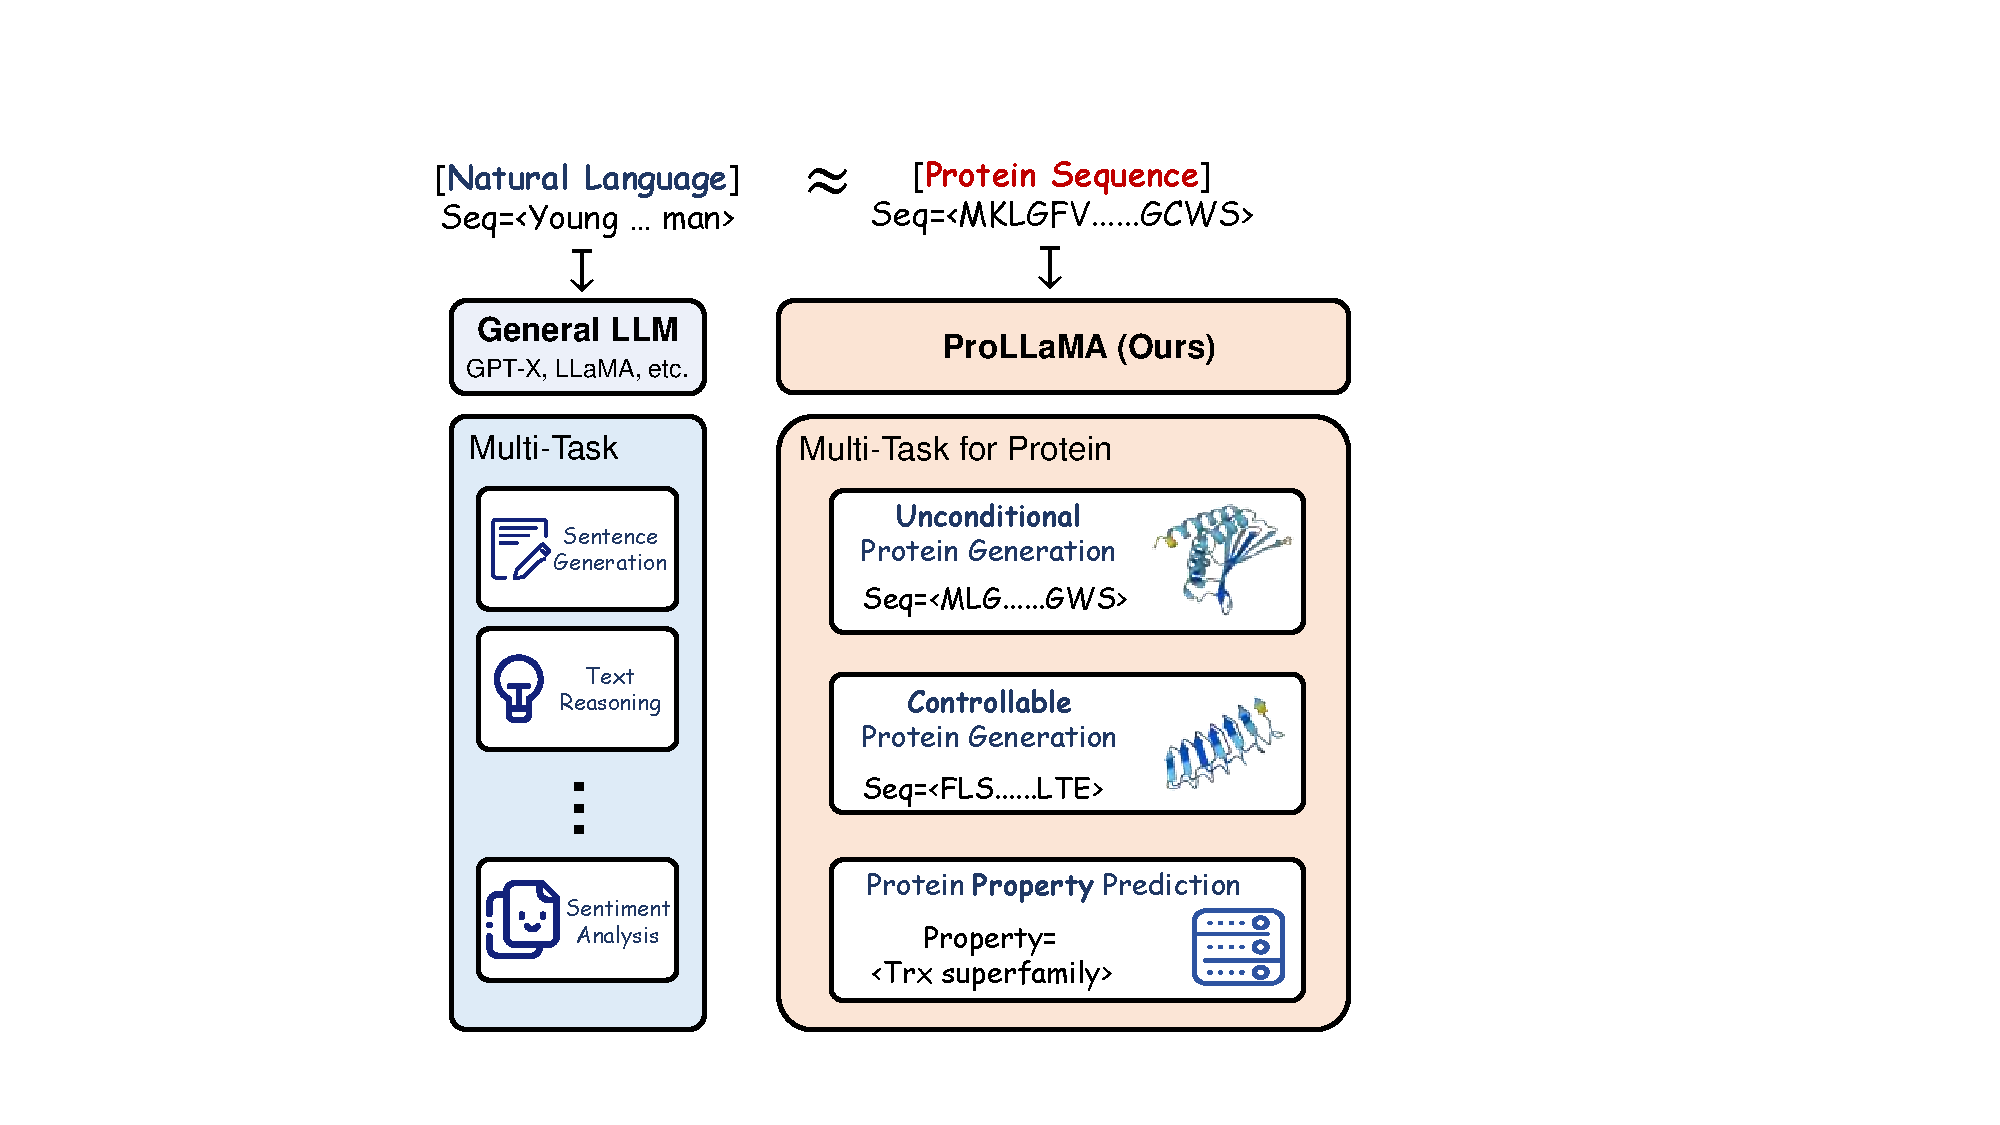
\includegraphics[scale=0.5]{images/multitask_LLMs_NLP_vs_PLP.pdf}
	\end{center}
	\credit{Image}{lv2024prollama}
\end{frame}

\begin{frame}{ProLLMs: Protein LLMs}
	\begin{itemize}\setlength\itemsep{1.5em}
		\item Protein sequences as the protein language
		\item PLP:Protein Language Processing~(\cite{bepler2021learning,ofer2021language})
		\item LLMs for protein design~(\cite{strokach2022deep,ferruz2022controllable})~
		\item Trained on vast protein corpus
		\item Pros: rapid generation of structurally plausible protein sequences
		\item Immense potential for biomedical and biotechnological innovations
		\item Challenge: extend capabilities beyond sequence generation
	\end{itemize}
\end{frame}

\begin{frame}[shrink=10]{Protein Language Models (PLMs)}
	\begin{itemize}\setlength\itemsep{1.5em}
		%\item ProLLMs $\subset$ PLMs
		\item[a.] Protein Large Language Model (ProLLM)
		\begin{itemize}
			\item Decoder-only
			\item Casual Language Modelling (CLM)
			\item Similar to general LLMs
			\item Tasks
			\begin{itemize}
				\item De novo protein sequence generation
				\\Models: DARK~(\cite{moffat2022design}), ProGPT2~(\cite{ferruz2022protgpt2}), ProGen~(\cite{madani2023large}), ProgGen2~(\cite{nijkamp2023progen2})
				\item Fitness prediction~(\cite{notin2022tranception})
			\end{itemize}
		\end{itemize}
		\item[b.] 
		\begin{itemize}
			\item Encoder-only
			\item Masked Language Modelling (MLM)
			\item Application: protein representation learning
			\item Downstream task: property prediction~(\cite{xu2023protst})
			\item Models
			\begin{itemize}
				\item ESM-1b~(\cite{rives2021biological})
				\item ProteinBERT~(\cite{brandes2022proteinbert})
				\item ESM-2~(\cite{lin2023evolutionary})
			\end{itemize}
		\end{itemize}
		\item[c.] 
		\begin{itemize}
			\item Encoder-decoder
			\item Sequence-to-Sequence (Seq2Seq)
			\item Models
			\begin{itemize}
				\item LM-DESIGN~(\cite{zheng2023structure})
				\\Tasks: De novo protein sequence generation
				\item ProLLaMA (this)
				\\Tasks: all the above
			\end{itemize}
		\end{itemize}
		\item Other models: \cite{yang2018learned}, UniRep~(\cite{alley2019unified}), MSA Transformer~(\cite{rao2021msa}), ProtTrans~(\cite{elnaggar2021prottrans})
	\end{itemize}
\end{frame}

\begin{frame}{Challenges}%Problem}
	\begin{itemize}\setlength\itemsep{1.5em}
		\item De novo design of long and structurally plausible protein
		sequences~(\cite{ferruz2022protgpt2}) %is highly challenging.
		\item Extend LLM capabilities beyond sequence generation
		\item Beyond protein language
		\begin{itemize}
			\item beyond protein sequences and co-evolutionary
			information
			\item need of protein function and property information
			\item protein language is not sufficient for some PLP tasks
			\begin{itemize}
				\item tasks: controllable protein generation, protein property prediction, \dots
				\item components: instruction (input), output
			\end{itemize}
			\item natural language ability~(\cite{xu2023protst,wang2023instructprotein})
		\end{itemize}
		\item Instruction following
		\item Training resource consumption
%		\begin{itemize}
%			\item Feasibility
%		\end{itemize}
	\end{itemize}
\end{frame}

\begin{frame}{Limitations in Current LLMs for Protein Language}
	\begin{itemize}\setlength\itemsep{3em}
		\item Single-task
		\item Lack Natural Language Capabilities
		\begin{itemize}
			\item Protein Language cannot fully represent all components of some tasks (User instruction, expected output)
		\end{itemize}
		\item Insufficient Instruction Understanding
		\item High Training Resource Demands
	\end{itemize}
\end{frame}

\begin{frame}{Goals}
\begin{itemize}\setlength\itemsep{3em}
	\item Protein engineering
	\item Protein fitness landscape understanding
	\item \cite{pan2021recent,ren2022proximal,song2023importance}
\end{itemize}
\end{frame}

\begin{frame}{ProLLaMA}
	\begin{itemize}
		\item Protein Language Processing
		\item Training Framework
		\begin{itemize}
			\item Any general LLM $\rightarrow$ ProLLM
			\item Two or More Stages
			\item Universal
			\item Efficient, low Overhead
			\item Scalable
		\end{itemize}
		\item Multi-tasking
		\begin{itemize}
			\item Unconditional Protein Sequence Generation
			\item Controllable Protein Sequence Generation
			\item Protein Property Prediction
			\item \dots
		\end{itemize}
		\item Language: Protein + Natural
		\item %Efficient Training: 
		LoRA: Low-Rank Adaptation~(\cite{hu2021lora})
		\begin{itemize}
			\item prevents catastrophic forgetting of natural language knowledge
			\item more scalability
			\item less training cost
		\end{itemize}
	\end{itemize}
\end{frame}

\begin{frame}{Model}
	\begin{center}
		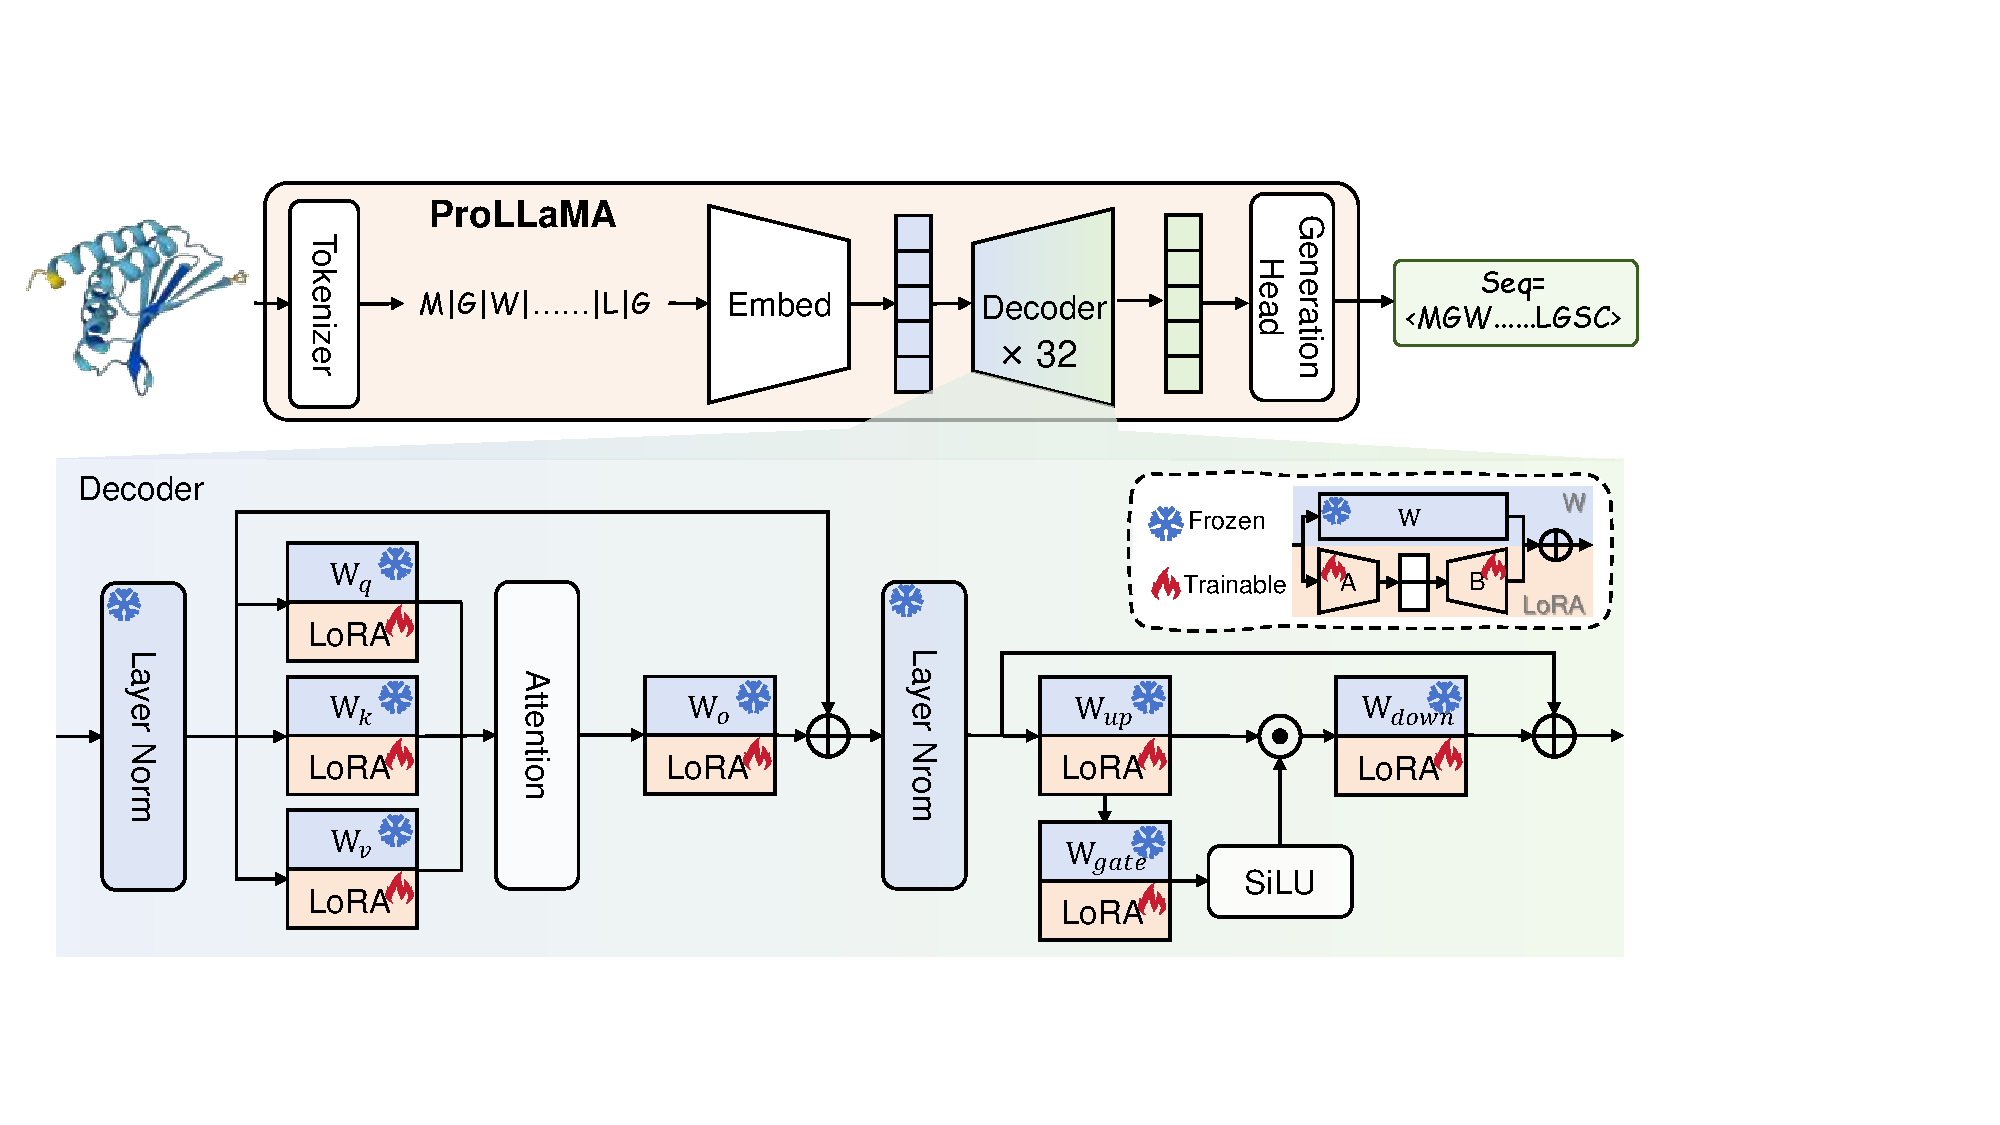
\includegraphics[scale=0.43]{images/model.pdf}
	\end{center}
	\credit{Image}{lv2024prollama}
	\begin{itemize}
		\item reuses pre-trained general LLM for NLP (e.g., LLaMA2)
		\item decoder: trains only LoRA, keeps everything else frozen
		\begin{itemize}
			\item preserves natural language abilities
		\end{itemize}
	\end{itemize}
\end{frame}

\begin{frame}[shrink=30]{Learning Stages}
	\begin{center}
		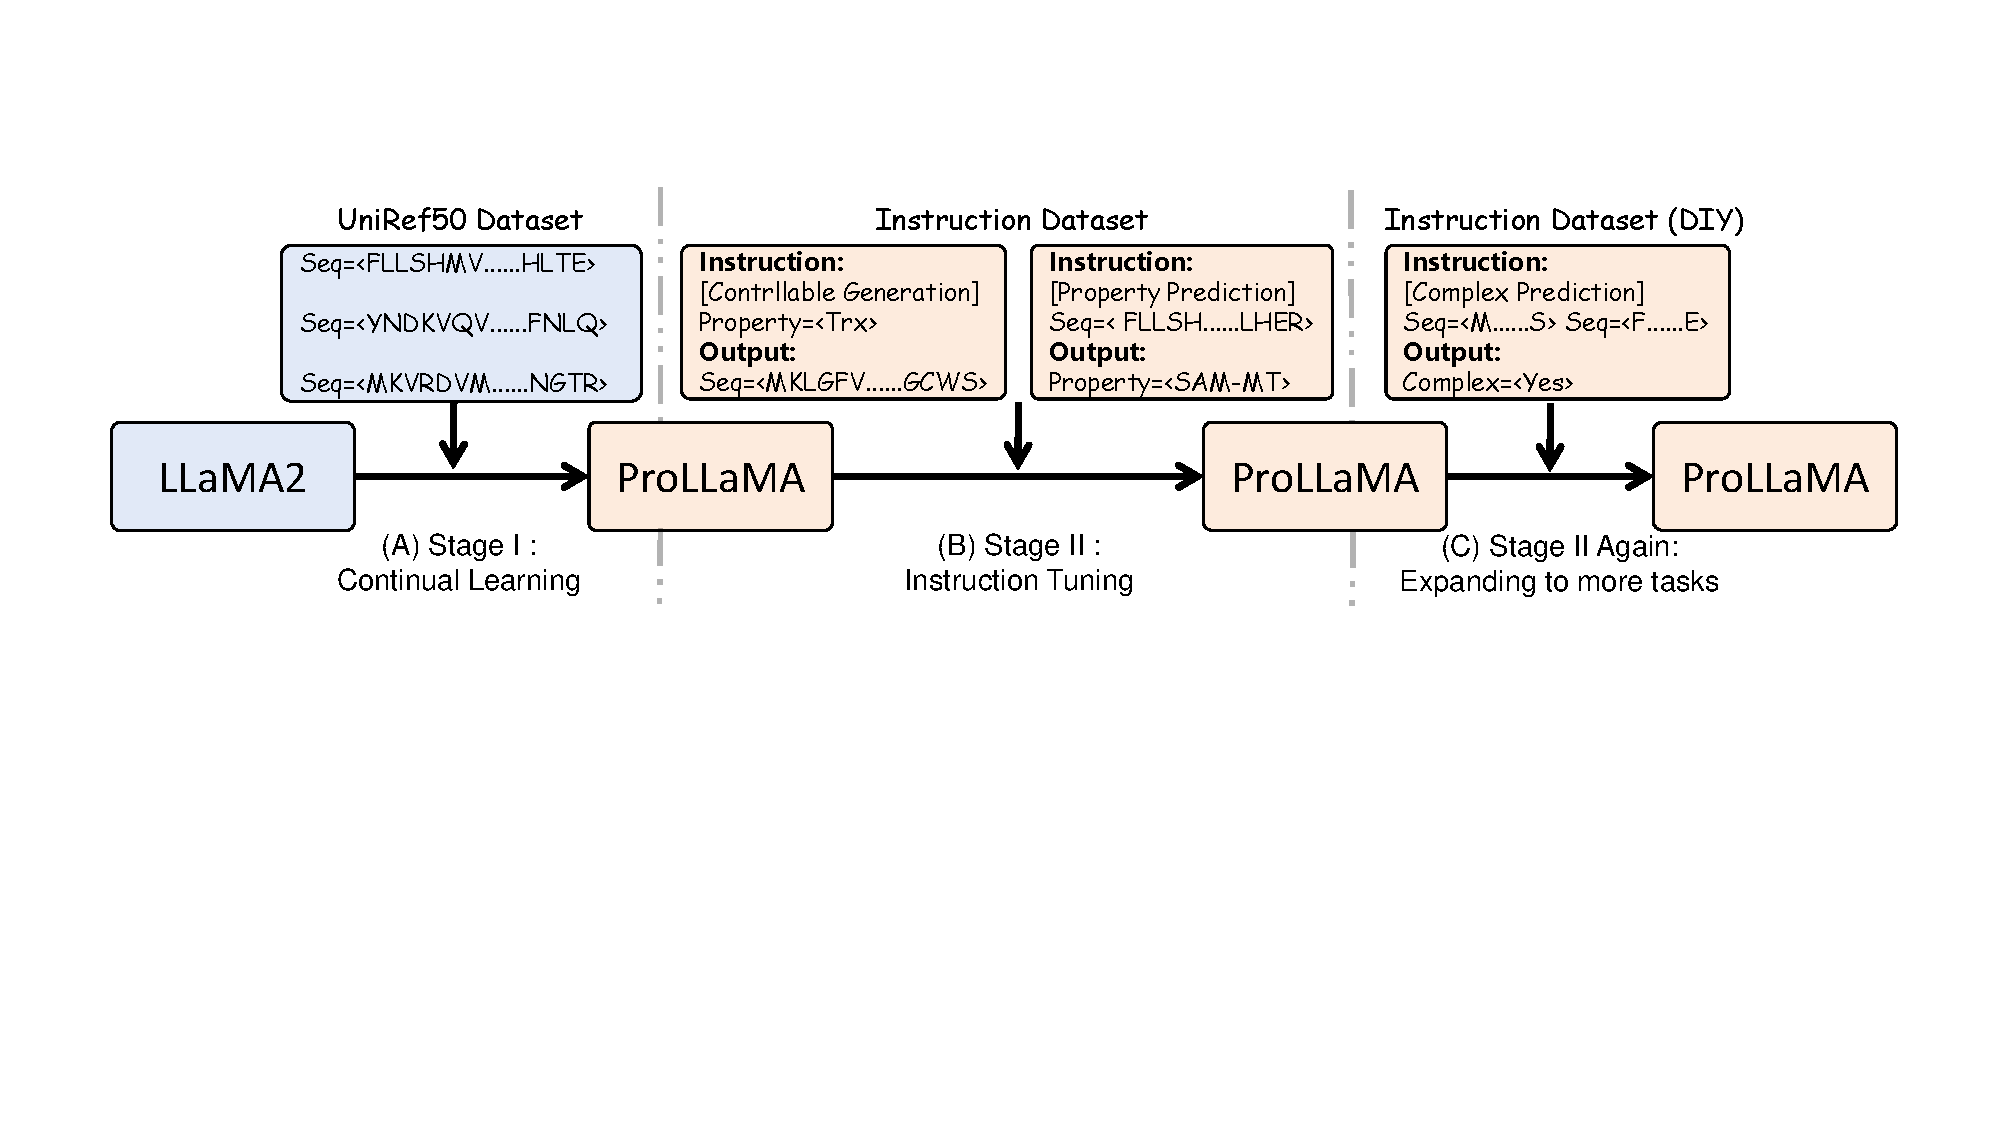
\includegraphics[scale=0.5]{images/training.pdf}
	\end{center}
	\credit{Image}{lv2024prollama}
	\begin{itemize}
		\item Stage I
		\begin{itemize}
			\item reuses pre-trained general LLM for NLP (e.g., LLaMA2)
			\item learns protein language
			\item trains decoder's LoRA
			\item includes both the Embed and Generation Head layers in training
			\begin{itemize}
				\item a token may have different meanings in protein
				sequences and natural languages, requiring distinct embeddings for the same token.
			\end{itemize}
		\end{itemize}
		\item Stage II
		\begin{itemize}
			\item learns to follow instructions
			\item multiple tasks
			\item trains only decoder's LoRA at a lower rank than Stage I
		\end{itemize}
		\item More stages
		\begin{itemize}
			\item optional
			\item more tasks
		\end{itemize}
		\item preserves natural language abilities
	\end{itemize}
\end{frame}

\begin{frame}[shrink=10]{Evaluation Metrics - Protein Generation}
	\begin{columns}
		\begin{column}{0.5\textwidth}
			\begin{itemize}\setlength\itemsep{1em}
				\item structural plausibility of a protein
				\begin{itemize}
					\item \textbf{pLDDT}: Local Distance Difference Test~(\cite{jumper2021highly})
					\begin{itemize}
						\item \red{Unreliable with Intrinsically Disordered Regions (IDRs)}
						\item Tool: OmegaFold
					\end{itemize}
					\item \textbf{SC-Perp}: Self-Consistency Perplexity~(\cite{alamdari2023protein})
					\begin{itemize}
						\item Tool: OmegaFold, ProteinMPNN
					\end{itemize}
				\end{itemize}
				\item structural similarity between generated and known proteins
				\begin{itemize}
					\item \textbf{TM-score}: Template Modeling score~(\cite{zhang2004scoring})
					\item \textbf{RMSD}:  Root-Mean-Square Deviation
					\begin{itemize}
						\item Atomic distance
					\end{itemize}
					\item Tool: Foldseek
					\item Reference Protein Databases: AFDB, PDB
				\end{itemize}
			\end{itemize}
		\end{column}
		\begin{column}{0.5\textwidth}
			\begin{itemize}\setlength\itemsep{1em}
				\item sequence similarity between generated and known proteins
				\begin{itemize}
					\item \textbf{Seq-Ident}: Sequence Identity
					\item Low = sequence diversity
					\item Tool: Foldseek
					\item Reference Protein Databases: AFDB, PDB
				\end{itemize}
				\item homology between generated and known proteins
				\begin{itemize}
					\item \textbf{H-Prob}: Homologous Probability
					\begin{itemize}\setlength\itemsep{1em}
						\item Probability that a generated protein is homologous to a known one
					\end{itemize}
					\item Homologous proteins have a common evolutionary origin, shared ancestry
					\item Tool: Foldseek
					\item Reference Protein Databases: AFDB, PDB
				\end{itemize}
			\end{itemize}
		\end{column}
	\end{columns}
	\vspace{1em}
	%What does homology mean?
	Note: since averages are considered, there are instances where generated proteins outperform natural proteins.
\end{frame}

\begin{frame}{Levels (Orders) of Protein Structure}
	\vspace{-0.5em}
	\begin{center}
		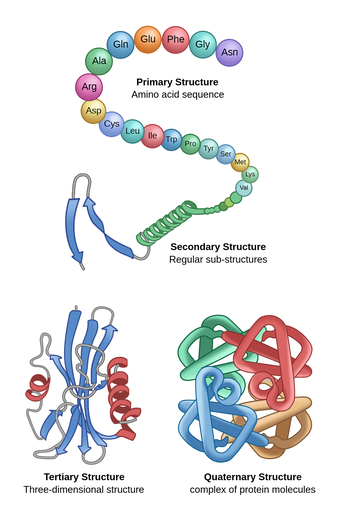
\includegraphics[trim={0 0 0 2em},clip,scale=0.46]{images/protein_structure_levels.png}
	\end{center}
	\vspace{-1.5em}
	\crediturl{Image}{https://theory.labster.com/protein-structure}
\end{frame}

\begin{frame}{Primary Protein Structure}
	\begin{center}
		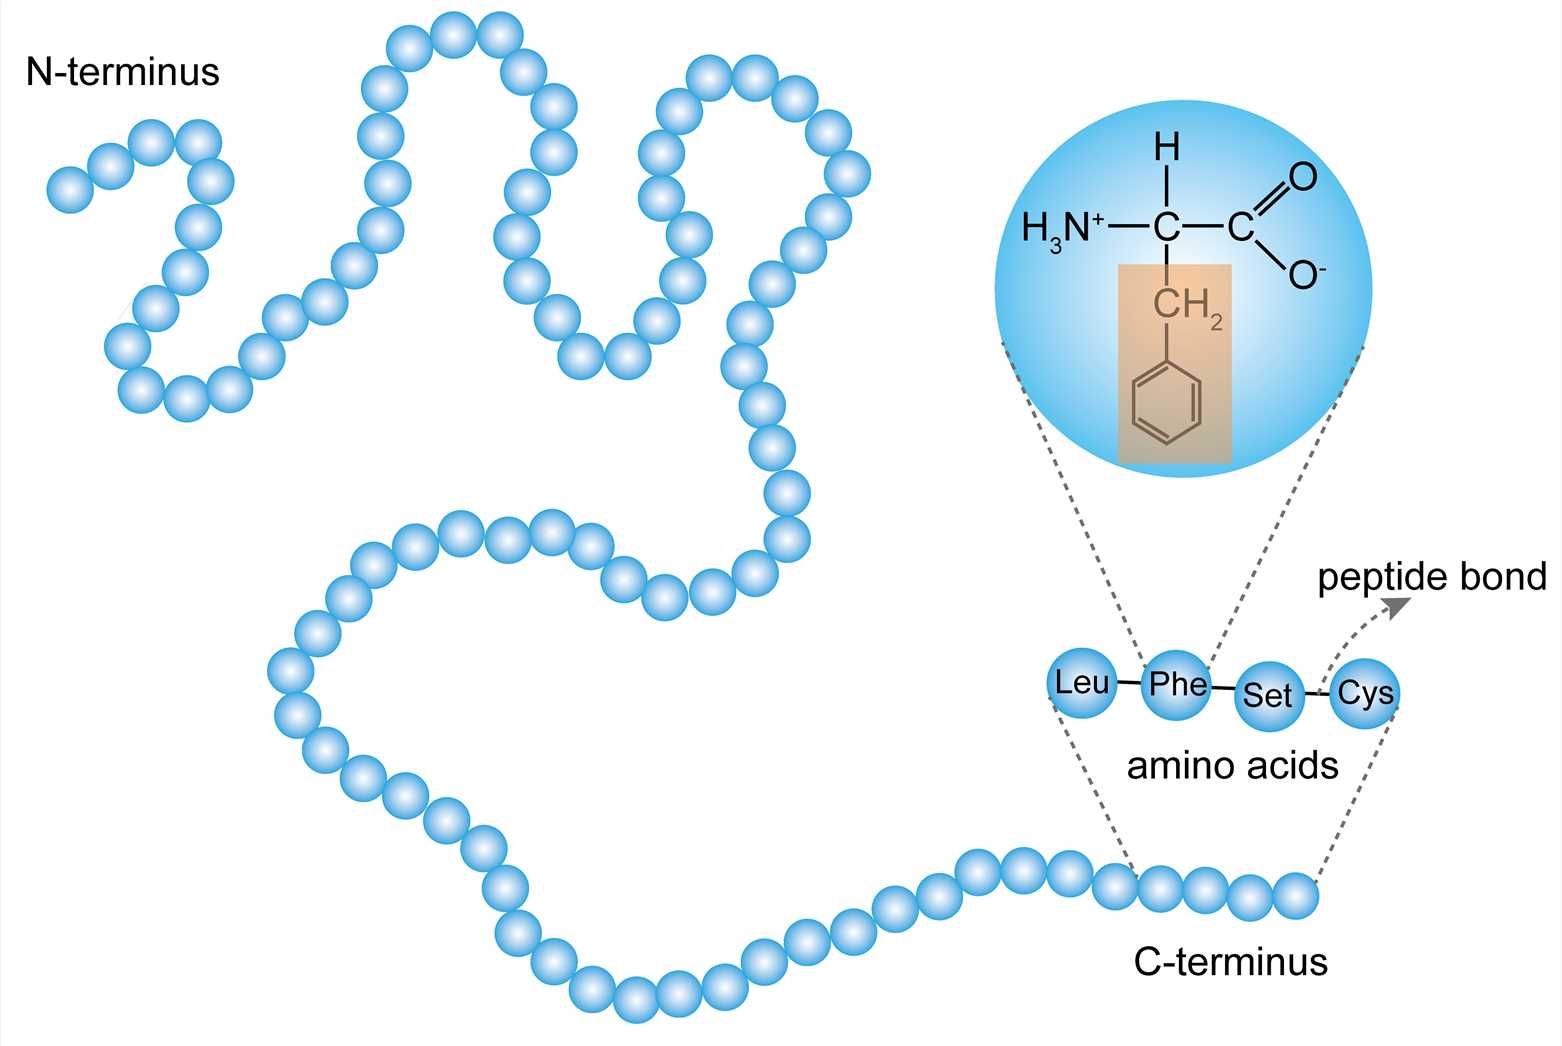
\includegraphics[scale=0.22]{images/primary_protein_structure.jpg}
	\end{center}
	\crediturl{Image}{https://www.creative-biostructure.com/levels-of-protein-structure.htm}
	\begin{itemize}
		\item One-dimensional sequence
		\item Chain of amino acids, polypeptide chain
		\item 20 possible amino acids
	\end{itemize}
\end{frame}

\begin{frame}{Secondary Protein Structure}
	\begin{center}
		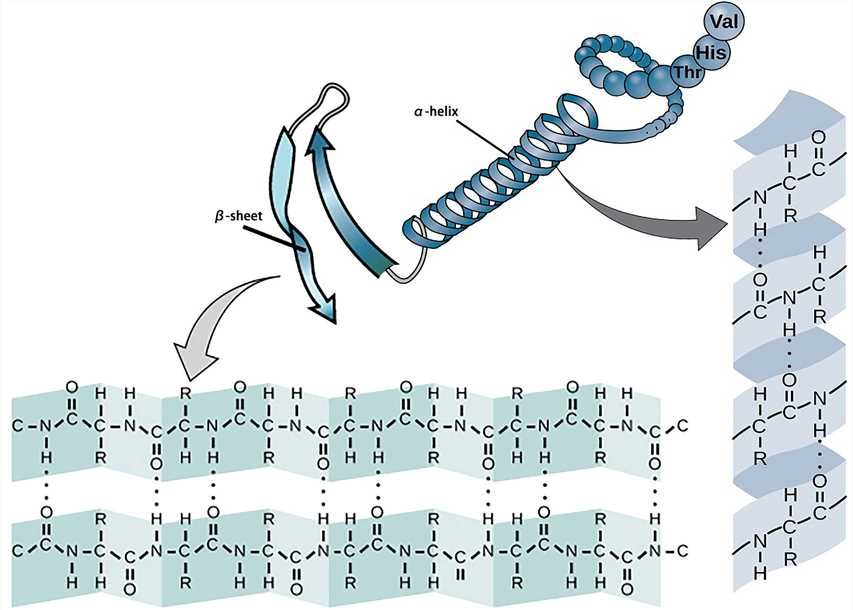
\includegraphics[scale=0.44]{images/secondary_protein_structure.jpg}
	\end{center}
	\crediturl{Image}{https://www.creative-biostructure.com/levels-of-protein-structure.htm}
	\begin{itemize}
		\item Protein sequence folds due to hydrogen bonds in the peptide backbone
	\end{itemize}
\end{frame}

\begin{frame}{Tertiary Protein Structure}
	\begin{center}
		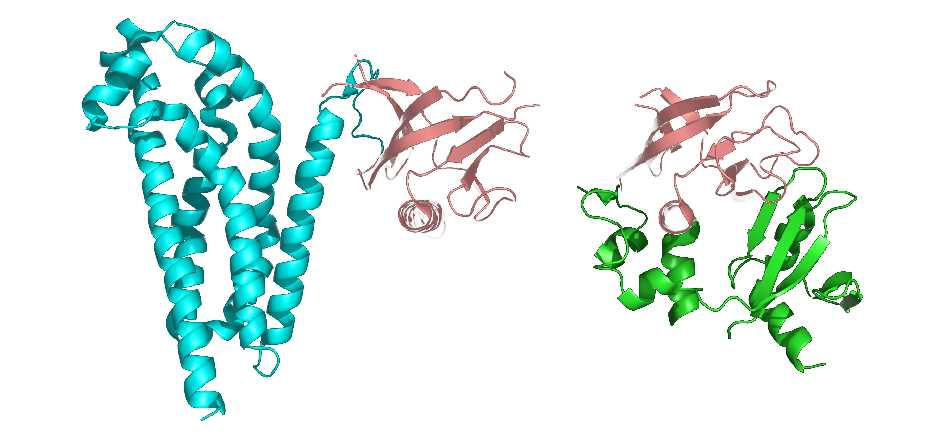
\includegraphics[scale=0.49]{images/tertiary_protein_structure.png}
	\end{center}
	\crediturl{Image}{https://www.creative-biostructure.com/levels-of-protein-structure.htm}
	\begin{itemize}
		\item Three-dimensional
		\item Protein folds and curls w.r.t. secondary structures due to side chain interactions
	\end{itemize}
\end{frame}

\begin{frame}{Quaternary Protein Structure}
\begin{center}
	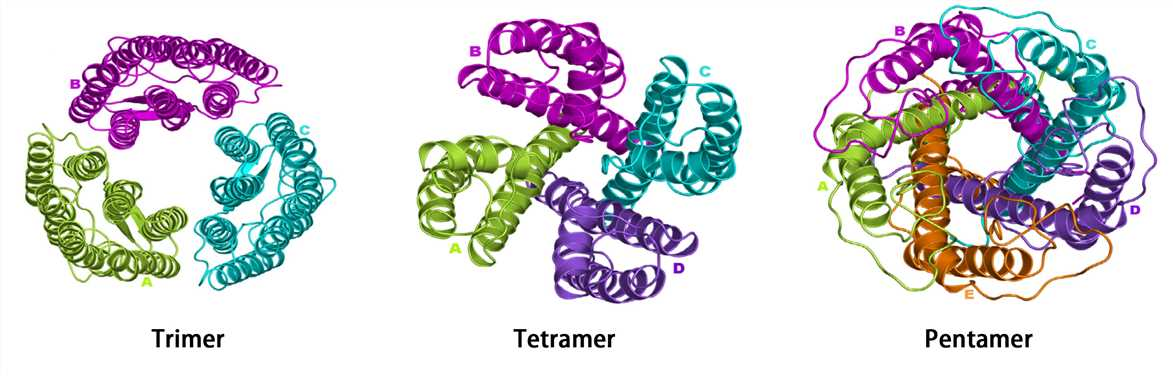
\includegraphics[scale=0.39]{images/quaternary_protein_structure.jpg}
\end{center}
\crediturl{Image}{https://www.creative-biostructure.com/levels-of-protein-structure.htm}
\begin{itemize}
	\item Composition of multiple polypeptide (amino acids) chains
	\item Only in some proteins
\end{itemize}
\end{frame}

\begin{frame}{Data Sources - Learning}
	\begin{itemize}\setlength\itemsep{3em}
		\item UniRef50: UniProt Reference Cluster 50~\cite{suzek2015uniref}
		\begin{itemize}
			\item Protein sequences
			\item Size: $>$10M
			\item Learning stages: continual learning, instruction tuning
			\item Tasks: unconditional and controllable protein generation
			\item sources: UniProtKB, UniParc
		\end{itemize}
		\item InterPro~\cite{paysan2023interpro}
		\begin{itemize}
			\item Functional analysis of proteins, classification into families, prediction of domains and important sites
			\item Protein property texts
			\item Size: $>$40k (entries), $>$400M (protein sequences)
			\item Learning stage: instruction tuning
			\item Task: protein property prediction
		\end{itemize}
	\end{itemize}
\end{frame}

\begin{frame}{Data Sources - Reference protein databases}
	\begin{itemize}\setlength\itemsep{3em}
		%\item Reference protein databases
		%\begin{itemize}
		\item PDB: Protein Data Bank~\cite{berman2002protein}
		\begin{itemize}
			\item Size: $>$200k
			\item Evaluation Metrics: TM-score, RMSD, H-Prob, and Seq-Ident
		\end{itemize}
		\item AFDB: AlphaFold Protein Structure Database~\cite{varadi2022alphafold}
		\begin{itemize}
			\item Size: $>$200M
			\item Evaluation Metrics: TM-score, RMSD, H-Prob, and Seq-Ident
		\end{itemize}
		%\end{itemize}
	\end{itemize}
\end{frame}

\begin{frame}{Preprocessing}
	\begin{itemize}
		\item adds specific prefixes and suffixes to each protein sequence
		\begin{itemize}\setlength\itemsep{1em}
			\item standardizes format
			\item reduces confusion
			\item aids (e.g., LLaMA2) in distinguishing the new protein language from its existing natural language knowledge
		\end{itemize}
	\end{itemize}
\end{frame}

\begin{frame}{Compared Models}
	\begin{itemize}
		\item CNN
		\begin{itemize}
			\item CARP~(\cite{alamdari2023protein})
			\begin{itemize}
				\item Task: Unconditional Protein Generation
			\end{itemize}
			\item LRAR~(\cite{alamdari2023protein})
			\begin{itemize}
				\item Task: Unconditional Protein Generation
			\end{itemize}
		\end{itemize}
		\item AutoEncoder
		\begin{itemize}
			\item ESM-1b~(\cite{rives2021biological})
			\begin{itemize}
				\item Tasks: Unconditional and Conditional Protein Generation
			\end{itemize}
			\item ESM-2~(\cite{lin2023evolutionary})
			\begin{itemize}
				\item Tasks: Unconditional and Conditional Protein Generation
			\end{itemize}
		\end{itemize}
		\item Diffusion
		\begin{itemize}
			\item EvoDiff~(\cite{alamdari2023protein})
			\begin{itemize}
				\item Tasks: Unconditional and Conditional Protein Generation
			\end{itemize}
		\end{itemize}
		\item LLM
		\begin{itemize}
			\item ProGPT2~(\cite{ferruz2022protgpt2})
			\begin{itemize}
				\item Tasks: Unconditional and Conditional Protein Generation
			\end{itemize}
			\item ProGen2~(\cite{nijkamp2023progen2})
			\begin{itemize}
				\item Tasks: Unconditional and Conditional Protein Generation
			\end{itemize}
		\end{itemize}
	\end{itemize}
\end{frame}

\begin{frame}{Performance in (Unconditional) Protein Generation}
	\begin{center}
		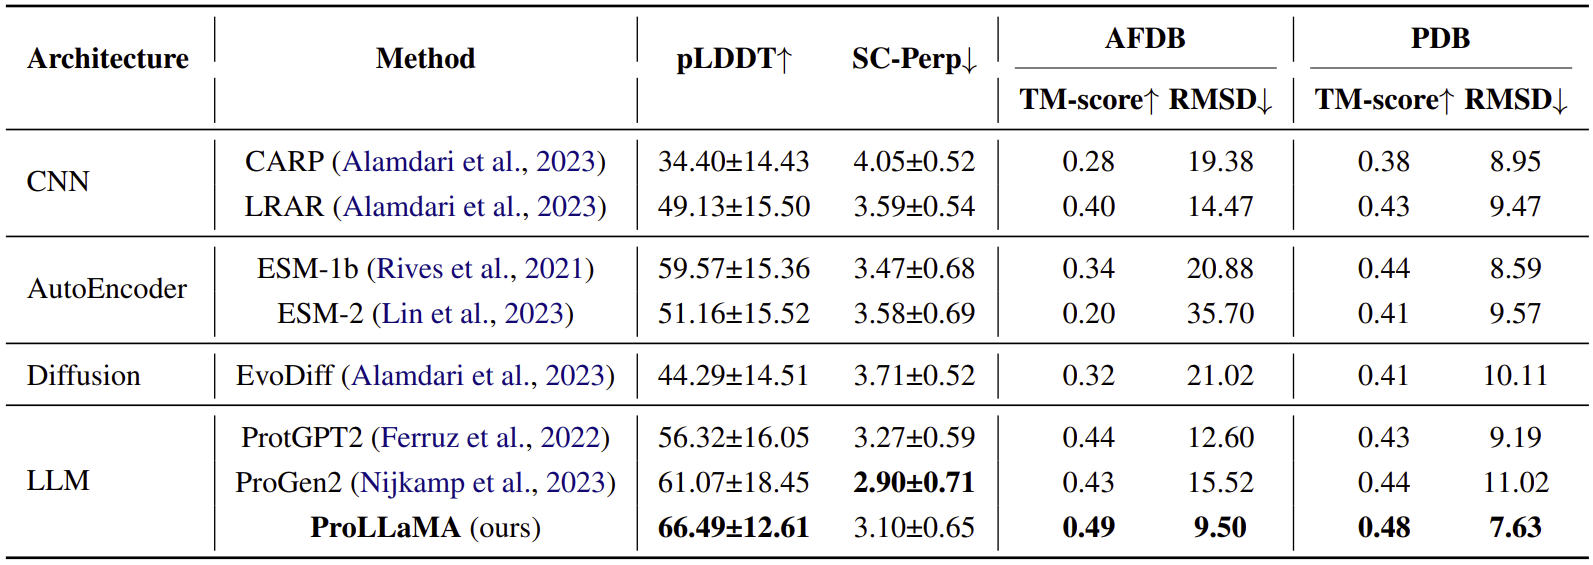
\includegraphics[scale=0.21]{tables/methods_comparison.png}
		\begin{tabular}{>{\centering\arraybackslash}p{11.7em}|>{\centering\arraybackslash}p{3.1em}>{\centering\arraybackslash}p{2.7em}|>{\centering\arraybackslash}p{2.3em}>{\centering\arraybackslash}p{2.3em}|>{\centering\arraybackslash}p{2.3em}>{\centering\arraybackslash}p{2.3em}}
			{\scriptsize \makecell{Natural protein \\ (\cite{alamdari2023protein})}} & \scalebox{.55}{\underline{68.25$\pm$17.85}} & \scalebox{.55}{3.09$\pm$0.63} & & & & \\\hline
		\end{tabular}
		\credit{(Modified) table}{lv2024prollama}
	\end{center}
	%\credit{Table}{lv2024prollama}
	\begin{itemize}
		\item ProLLaMA can generate proteins
		\begin{itemize}
			\item structurally plausible
			\item comparable to natural proteins
		\end{itemize}
	\end{itemize}
\end{frame}

\begin{frame}{Quality of Generated Protein w.r.t. Length}%ProLLaMA vs. ESM2 (Baseline) Model}
%\begin{center}
\begin{columns}
	\begin{column}{0.5\textwidth}
		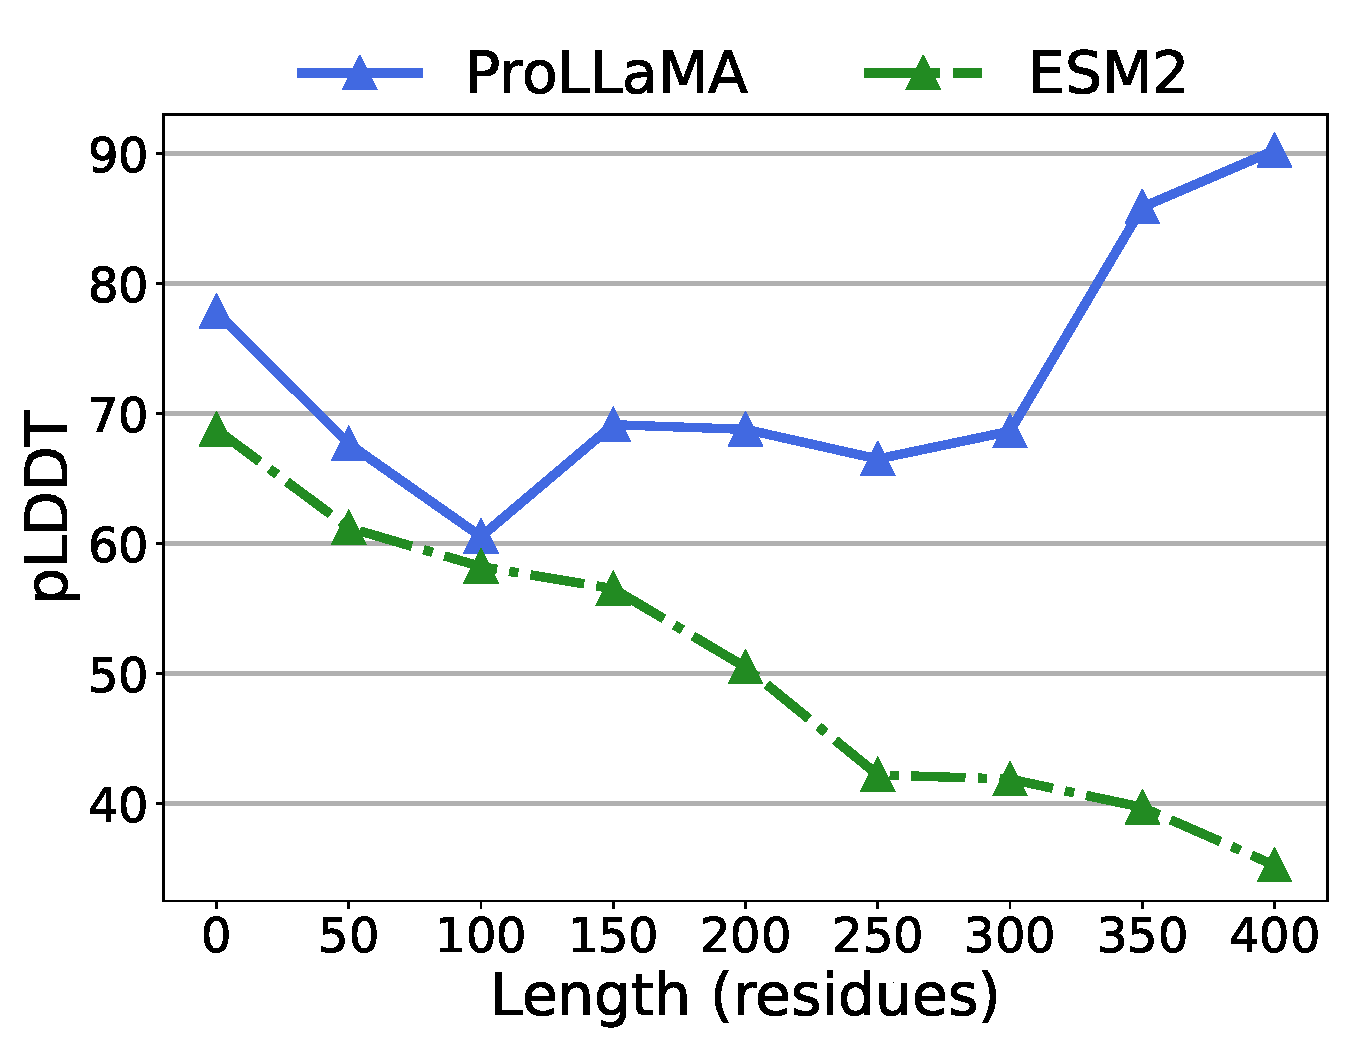
\includegraphics[scale=0.23]{images/combined_length_plddt_zhexiantu.pdf}
		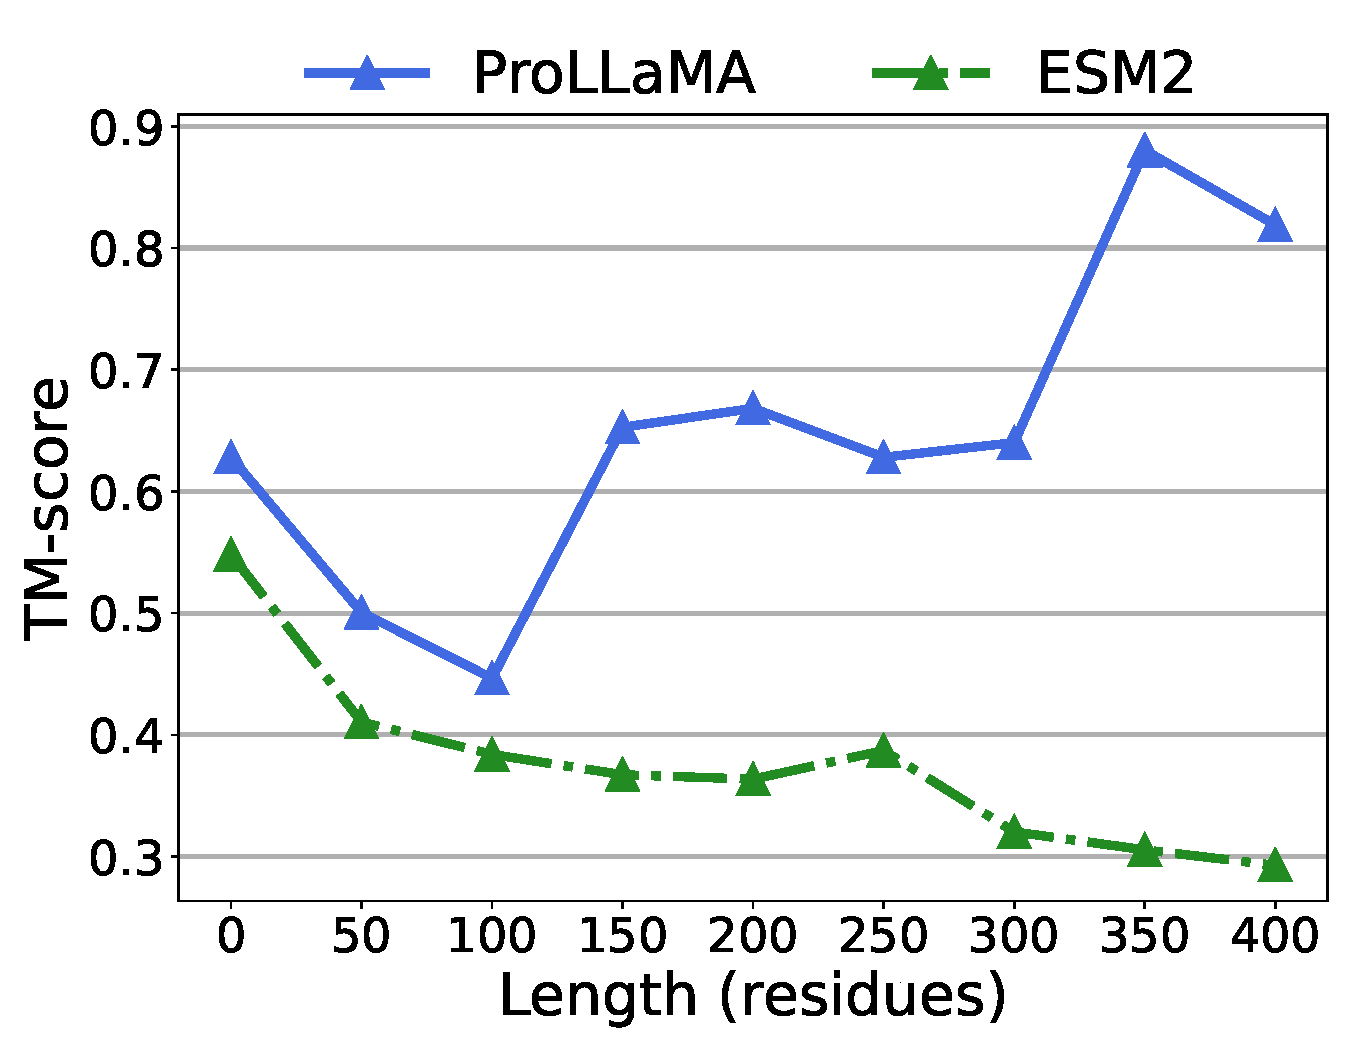
\includegraphics[scale=0.23]{images/combined_length_alntmscore_zhexiantu.pdf}
	\end{column}
	\begin{column}{0.5\textwidth}
		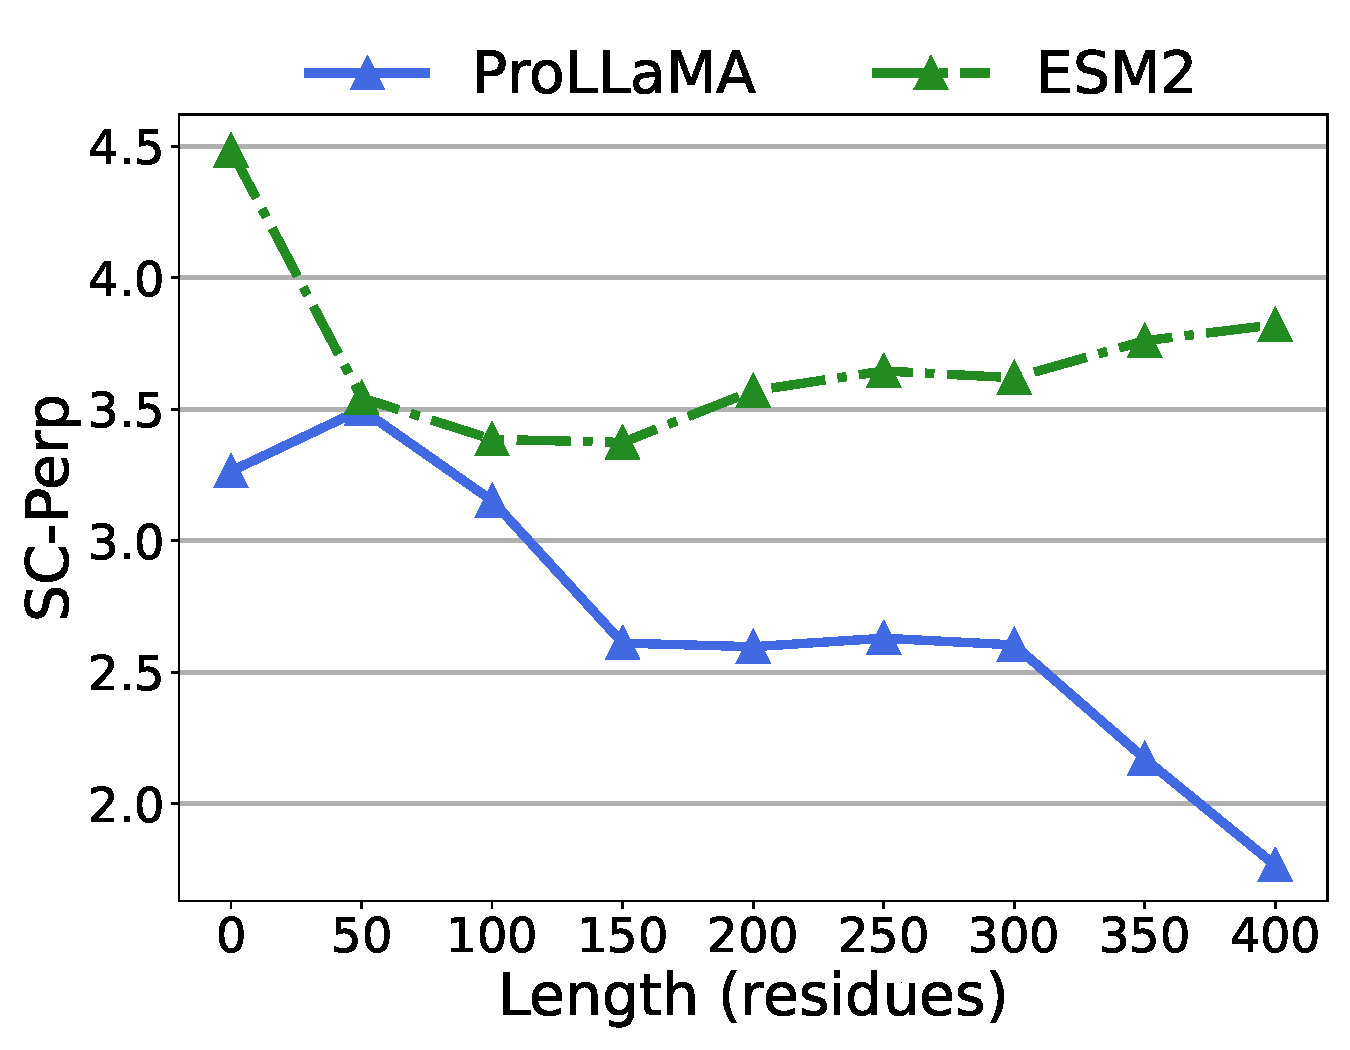
\includegraphics[scale=0.23]{images/combined_length_scperp_zhexiantu.pdf}
		\begin{itemize}
			\item ProLLaMA can capture long-range dependencies between amino acids.
		\end{itemize}
	\end{column}
\end{columns}
%\end{center}
\vspace{-2em}\credit{Image}{lv2024prollama}
\end{frame}

\begin{frame}{Performance in Controllable Protein Generation}% on Four Different Instructions
	\begin{center}
		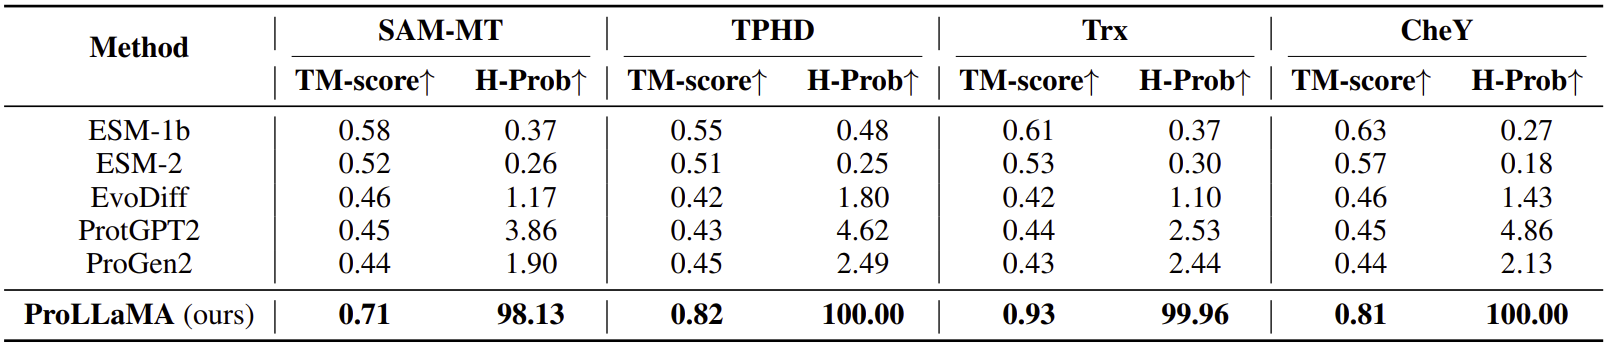
\includegraphics[scale=0.21]{tables/controlled_generation_comparison.png}
	\end{center}
	\vspace{-1em}\credit{Table}{lv2024prollama}
	\begin{itemize}
		\item ProLLaMA
		\begin{itemize}
			\item can generate protein sequences with desired functionalities
			\item Structures of generated proteins closely resemble those of natural proteins in the same superfamily, implying functional similarity.
			\item Generated proteins are homologous to natural ones and belong to the same superfamily.
		\end{itemize}
		\item Other models: much less controllable generation of proteins
		\item Superfamily descriptors: SAM-MT, TPHD, Trx, CheY
	\end{itemize}
\end{frame}

\begin{frame}{Controllable Generated vs. Natural Protein}
	\begin{columns}
		\begin{column}{0.5\textwidth}
			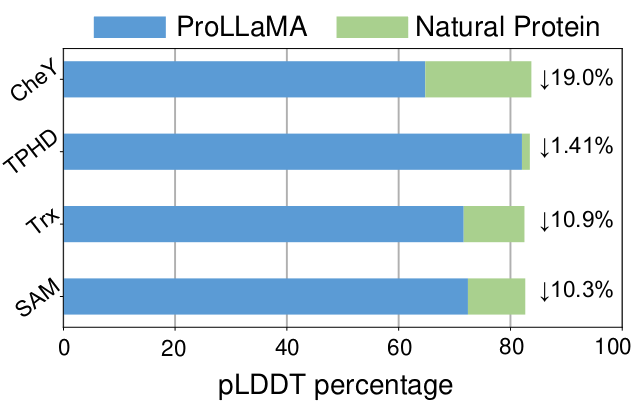
\includegraphics[scale=0.7]{images/d.png}
			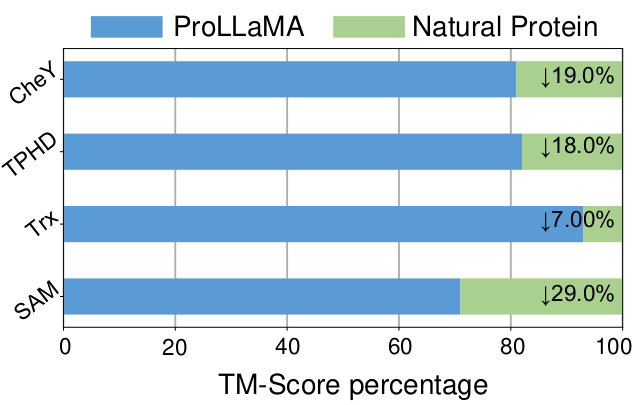
\includegraphics[scale=0.7]{images/f.png}
		\end{column}
		\begin{column}{0.5\textwidth}
			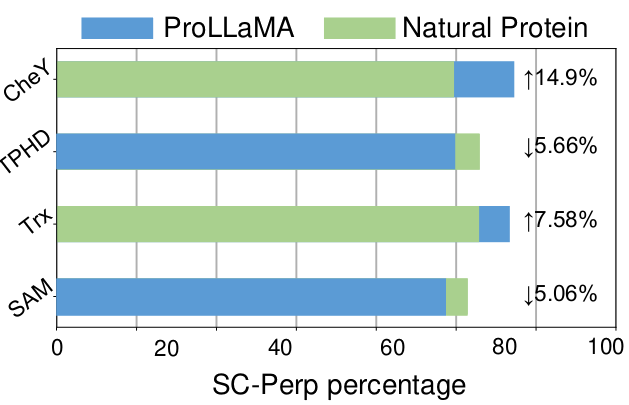
\includegraphics[scale=0.7]{images/e.png}
			\begin{itemize}
				\item Proteins generated by ProLLaMA are comparable to their
				natural counterparts in the same superfamily.
			\end{itemize}
		\end{column}
	\end{columns}
	\credit{Image}{lv2024prollama}
\end{frame}

\begin{frame}[shrink=1]{Visualization of Controllable Generated vs. Natural Proteins}
	\begin{center}
		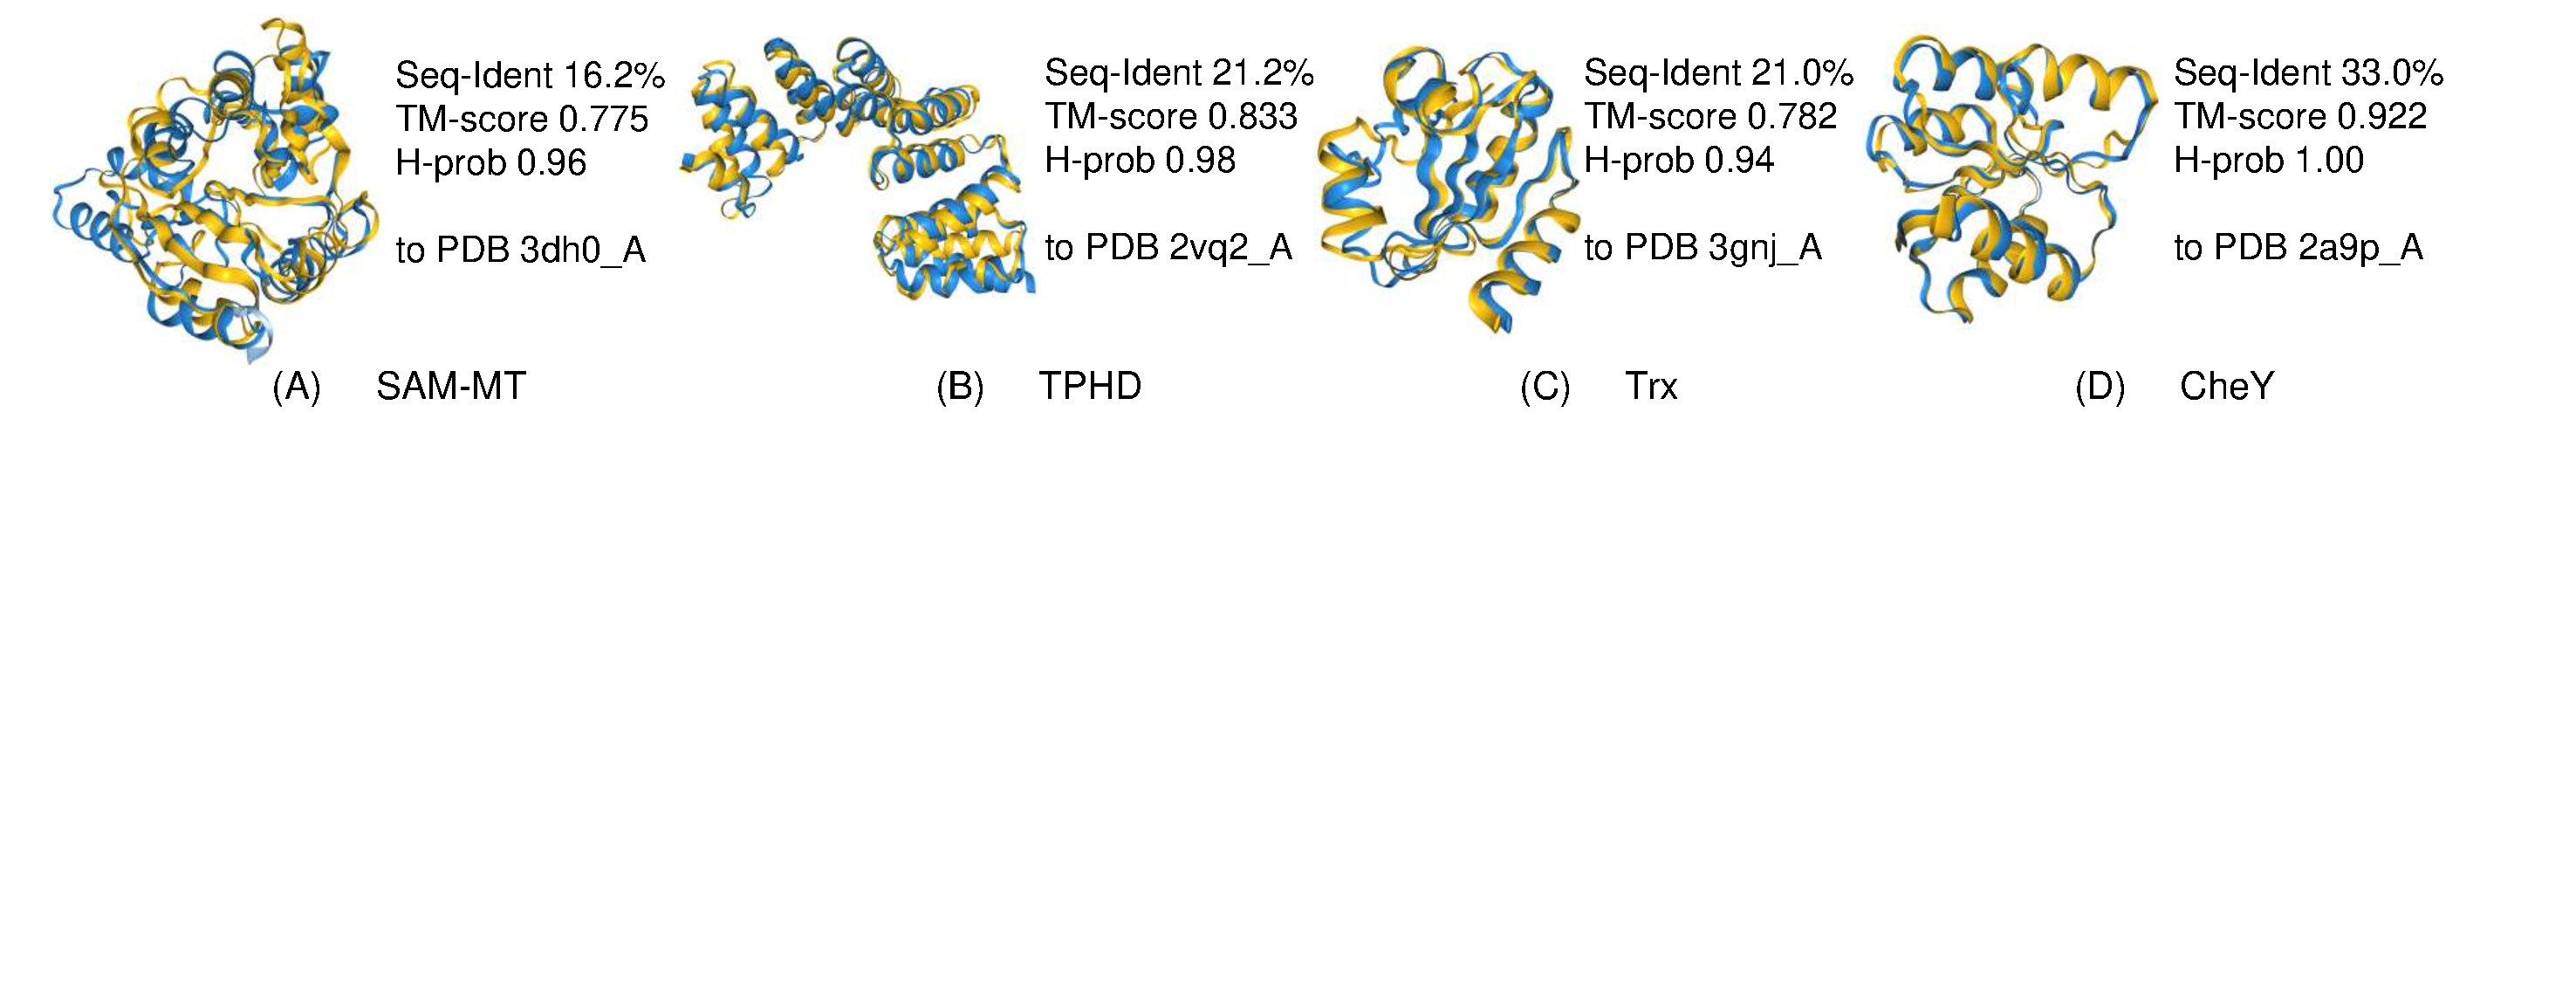
\includegraphics[trim={0 0 90em 0},clip,scale=0.4]{images/protein_visualization.pdf}
		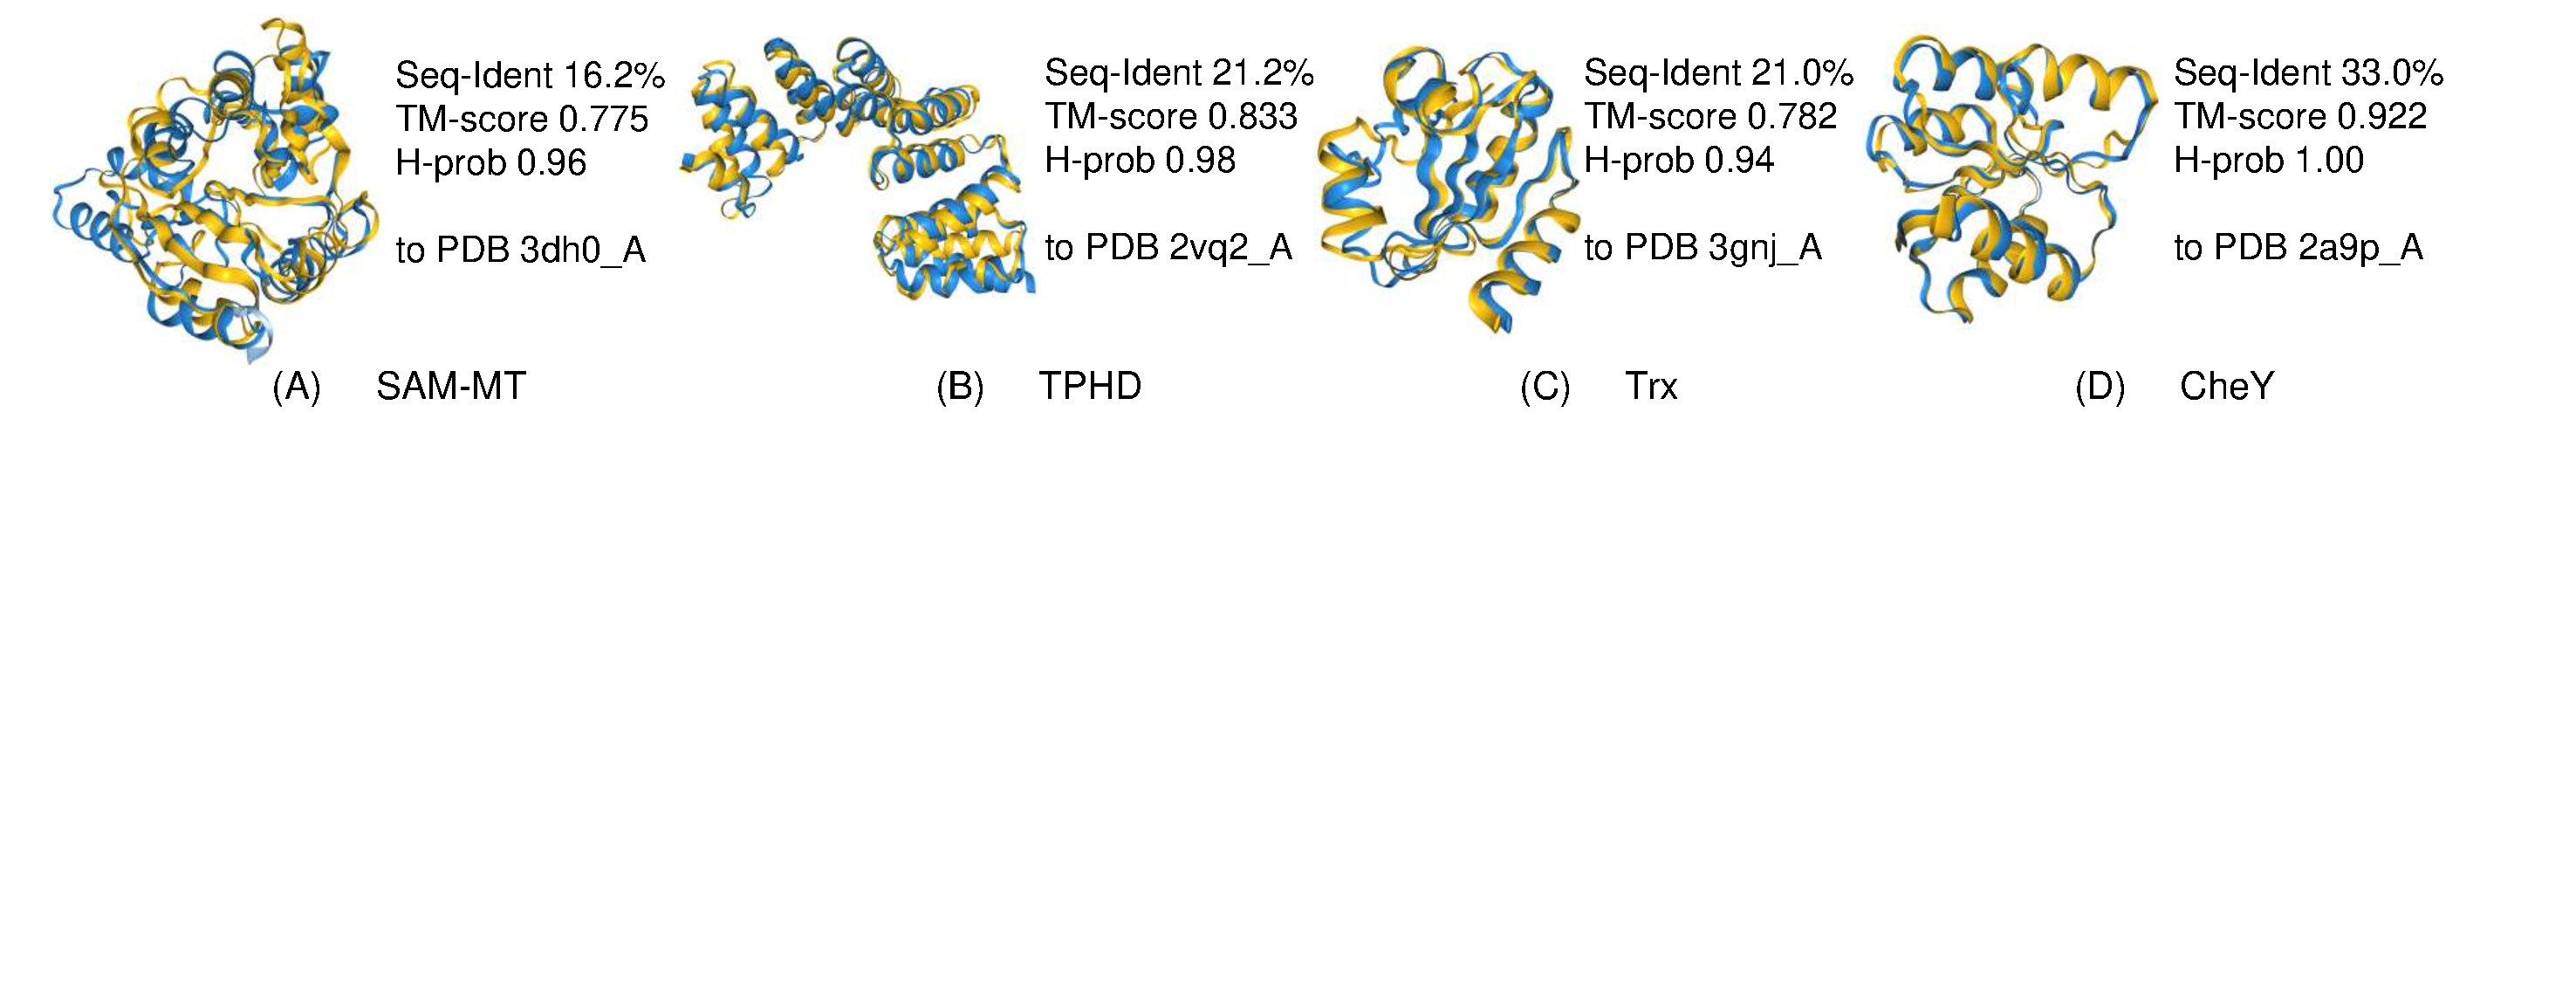
\includegraphics[trim={31.5em 0 57.4em 0},clip,scale=0.4]{images/protein_visualization.pdf}
		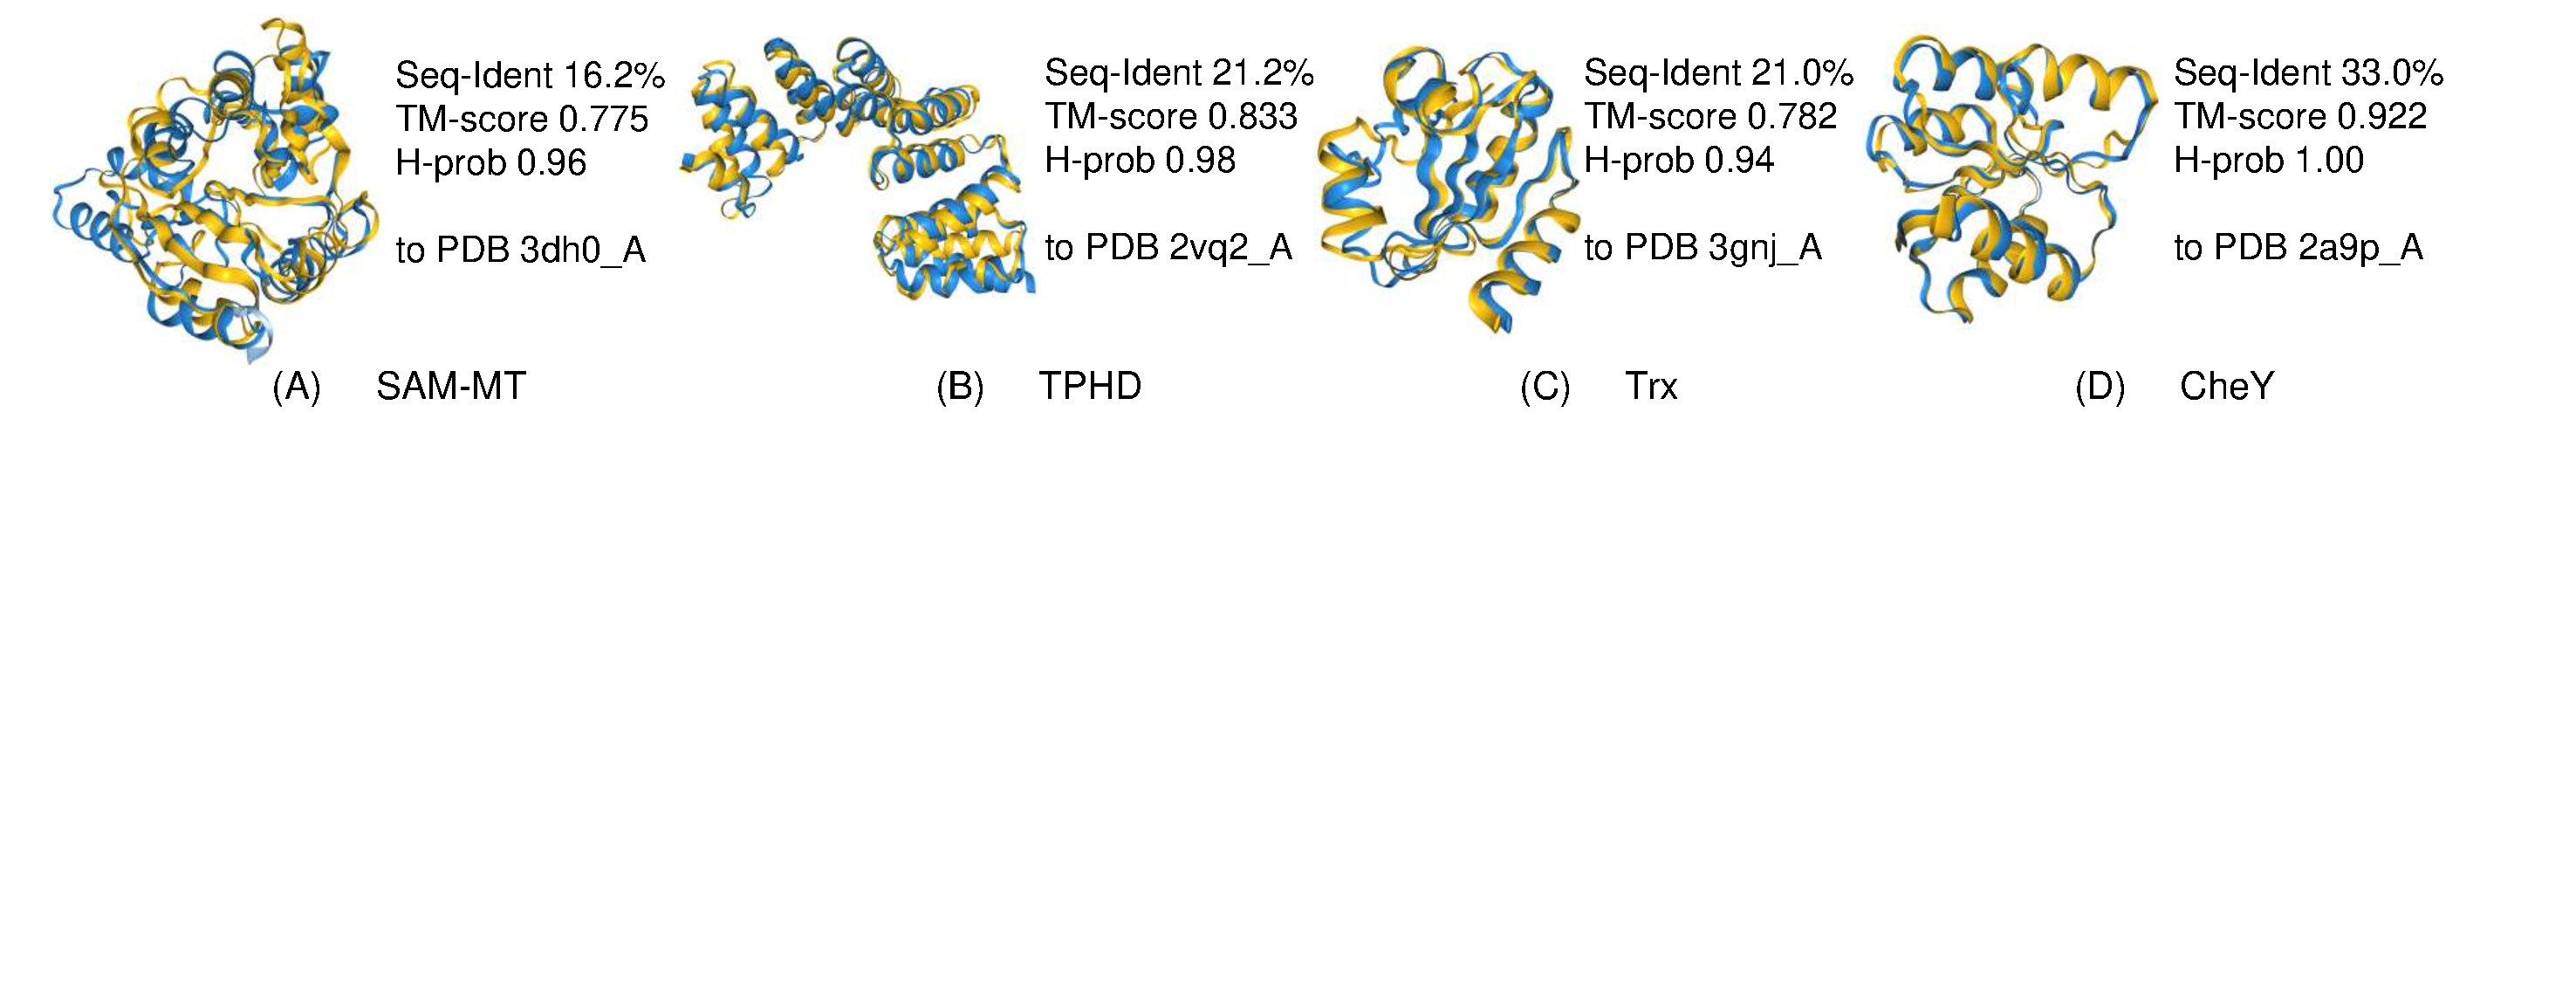
\includegraphics[trim={64em 0 30em 0},clip,scale=0.4]{images/protein_visualization.pdf}
		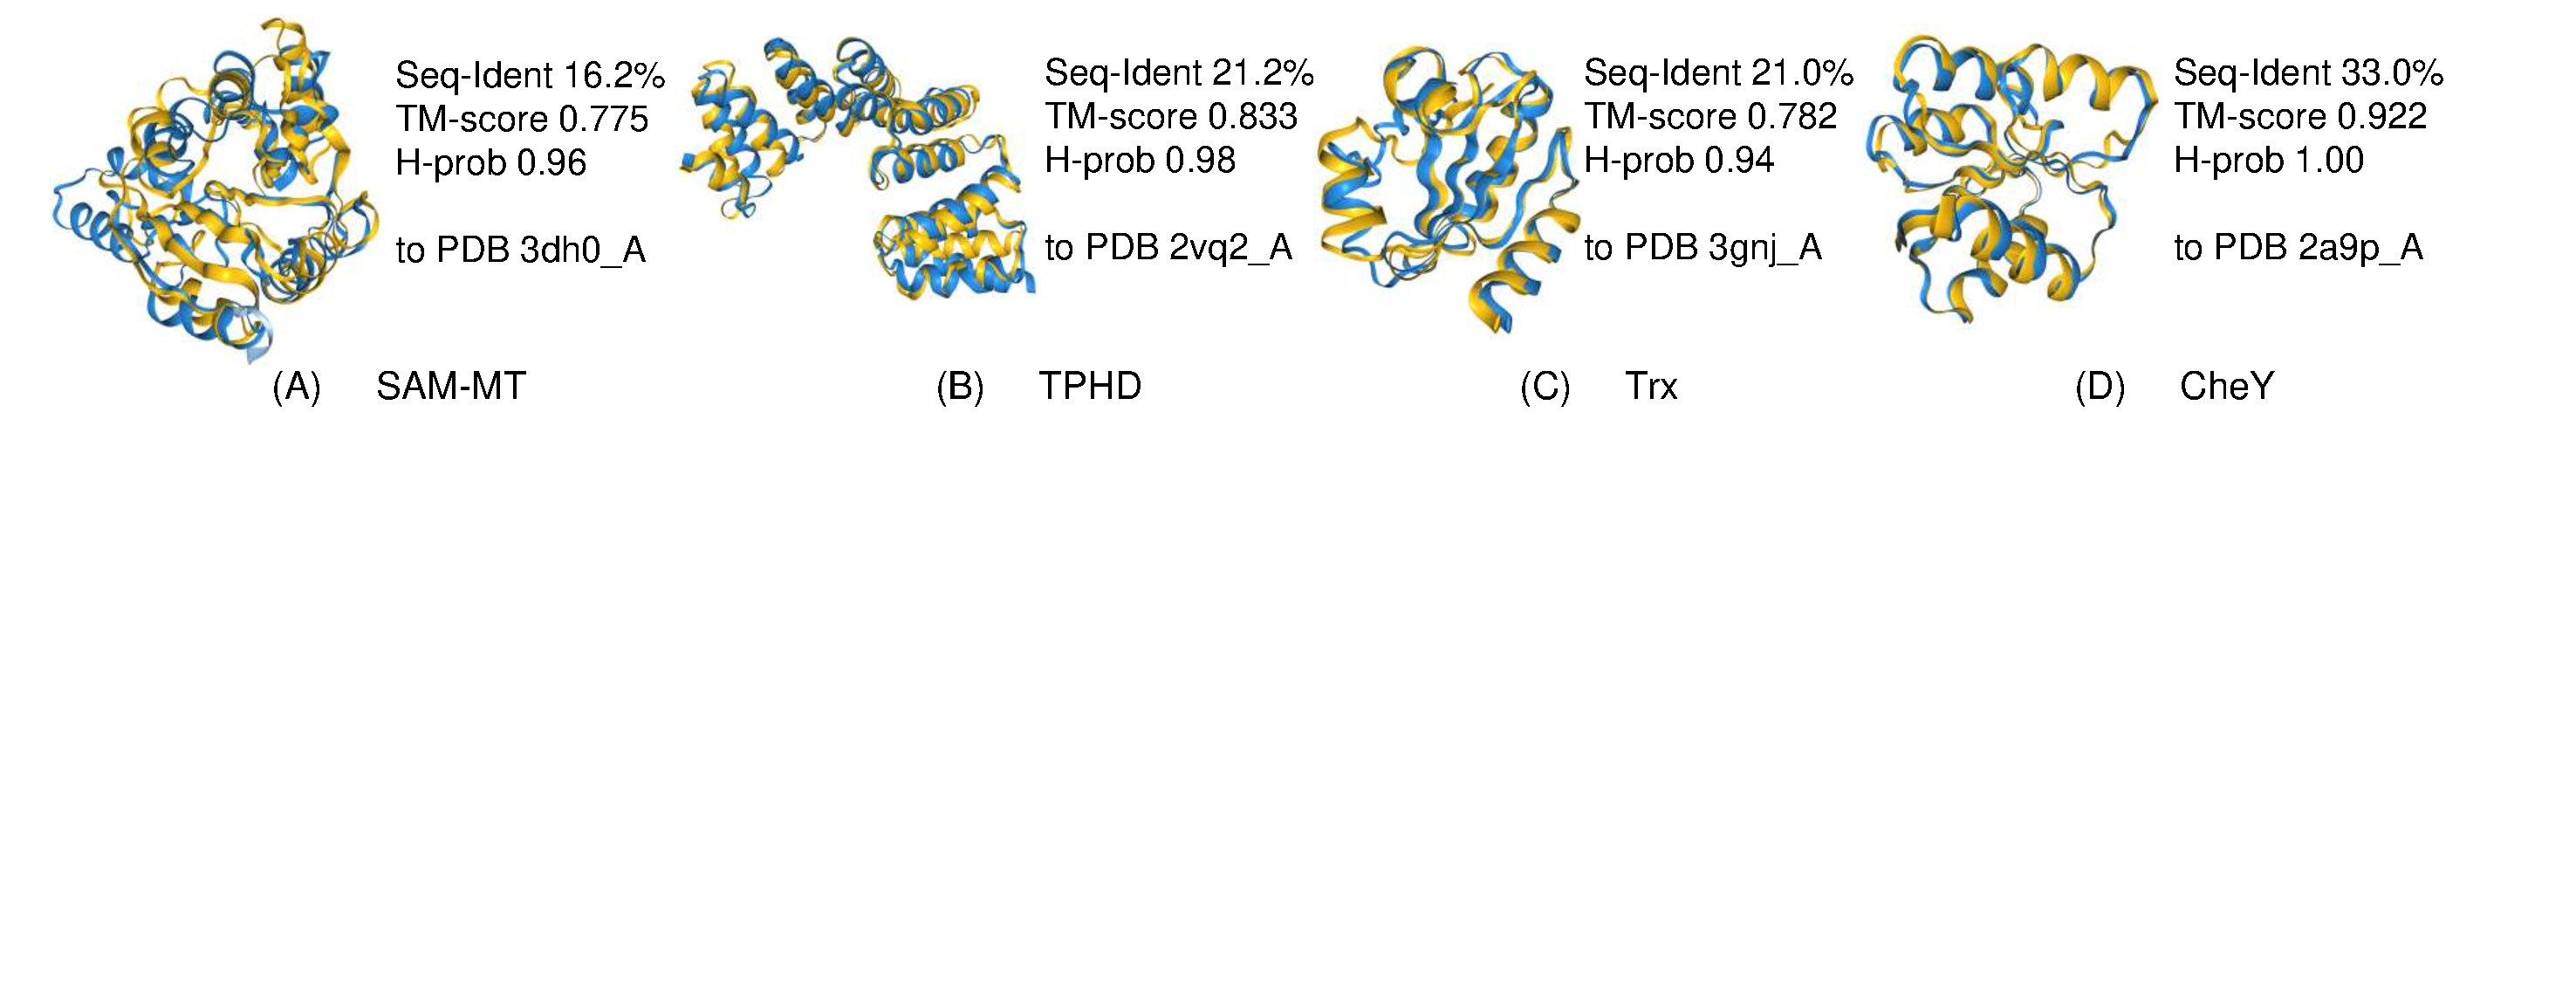
\includegraphics[trim={92em 0 0 0},clip,scale=0.4]{images/protein_visualization.pdf}
	\end{center}
	\vspace{-1em}\credit{Image}{lv2024prollama}
	\begin{itemize}
		\item Blue: generated proteins by superfamily, yellow: the most structurally similar natural proteins (counterparts) from PDB
		\item Generated and natural proteins belong to the same superfamily (source: InterPro)
		\item Similar in structure (function), different in sequence (novel)
	\end{itemize}
\end{frame}

\begin{frame}{Performance in Protein Property Prediction}
%	\begin{columns}
%		\begin{column}{0.5\textwidth}
%			\begin{center}
%				\begin{tabular}{cc}\hline
%					Property & Accuracy (\%) \\\hline
%					OBFD     & 100 \\
%					UPF0145  & 100 \\
%					NACD     & 100 \\
%					U3S      & 100 \\
%					CCHC     & 95.24  \\
%					Kazal    & 100 \\
%					SAM-MT   & 93.67  \\
%					TPHD     & 90.84  \\
%					Trx      & 94.17  \\
%					CheY     & 100 \\\hline
%				\end{tabular}
%			\end{center}
%			\credit{Table}{lv2024prollama}
%		\end{column}
%		\begin{column}{0.5\textwidth}
		\begin{itemize}
			\item 72\% average test accuracy
			\item $\sim$100\% test accuracy in many superfamilies
			\item 10k test examples
			\item One protein may belong to multiple superfamilies.
			\item (Multi-label) Accuracy Metric
			\begin{equation}
				\frac{\sum_{i=1}^N|Y_i \cap \hat{Y_i}|}{\sum_{i=1}^N|\hat{Y_i}|}
			\end{equation}
			\begin{itemize}
				\item $Y_i$, $\hat{Y_i}$: true and predicted property (superfamily) sets
			\end{itemize}
			\item ProLLaMA outputs a full textual description of the result.
		\end{itemize}
%		\end{column}
%	\end{columns}
\end{frame}

\begin{frame}{Natural Language Need}
	\begin{itemize}\setlength\itemsep{3em}
		\item Natural Language $\neq$ Protein Sequences
		\begin{itemize}\setlength\itemsep{1em}
			\item Natural language is \underline{complete} for NLP tasks
			\begin{itemize}
				\item Natural language can represent all \emph{components} for NLP tasks
				\\$\cdot$ \emph{components}: input instructions, expected output
			\end{itemize}
			\item Protein language is \underline{NOT complete} for PLP tasks
		\end{itemize}
		\item Example: protein property prediction task
		\begin{itemize}
			\item task instruction: ``Predict the property of this protein: MAFCF...FEV''
			\item expected output: ``The property is Trx superfamily.''
		\end{itemize}
	\end{itemize}
\end{frame}

\begin{frame}{Natural Language Ability}
	\begin{center}
		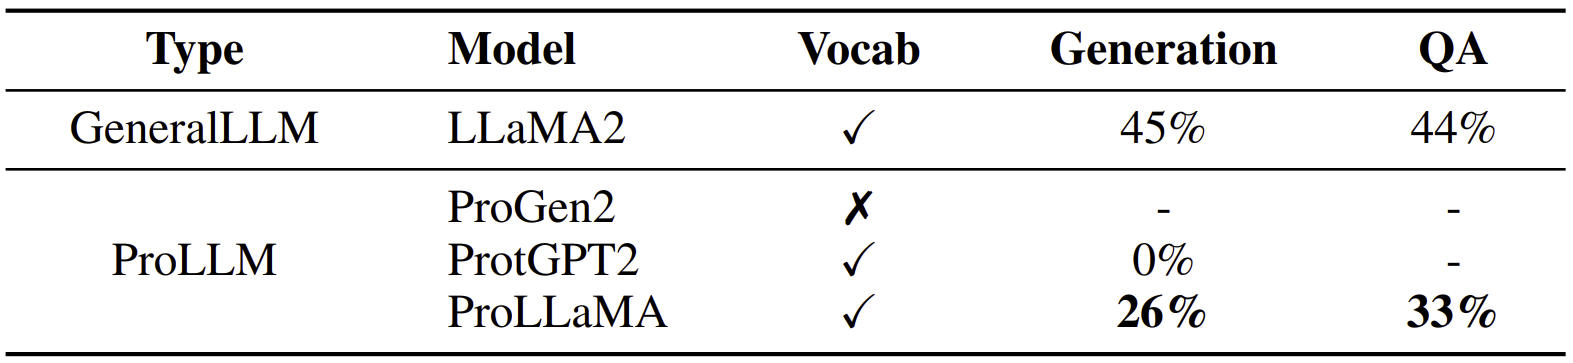
\includegraphics[scale=0.21]{tables/natural_language_ability_comparison.png}
	\end{center}
	\credit{Table}{lv2024prollama}
	\begin{itemize}
		\item Sentence generation on Wikipedia text
	\end{itemize}
\end{frame}

\begin{frame}{Summary}
	\begin{itemize}
		\item Protein Language Processing
		\item Training Framework
		\begin{itemize}
			\item Any general LLM $\rightarrow$ ProLLM
			\item Two or More Stages
			\item Universal
			\item Efficient, low Overhead
			\item Scalable
		\end{itemize}
		\item Multi-tasking
		\begin{itemize}
			\item Unconditional Protein Sequence Generation
			\item Controllable Protein Sequence Generation
			\item Protein Property Prediction
			\item \dots
		\end{itemize}
		\item %Efficient Training: 
		Low-Rank Adaptation (LoRA)
		\begin{itemize}
			\item Less Forgetting
			\item Less Training Cost
			\item More Scalability
		\end{itemize}
	\end{itemize}
\end{frame}
%\begin{frame}{Summary}
%	\begin{itemize}\setlength\itemsep{3em}
	%		\item Efficient training framework
	%		\item Can transform any general LLM into a multi-task ProLLM
	%		\item Versatility
	%		\begin{itemize}
		%			\item Unconditional protein generation
		%			\item Controllable protein generation
		%			\begin{itemize}
			%				\item Generates desired proteins with functions and structures similar to natural proteins, yet with novel sequences.
			%			\end{itemize}
		%			\item Protein property prediction
		%		\end{itemize}
	%		\item Exceptional performances
	%	\end{itemize}
%\end{frame}

\begin{frame}{Open questions}
	\begin{itemize}\setlength\itemsep{0.75em}
		\item Are current ProLLMs really unable to follow instructions? How did ProLLaMA authors realize that?
		\item Why does the quality of proteins generated by ProLLaMA increase as their sequence length increases? Why does ESM2 behave in the opposite way? What about other models?
		\item Isn't there any better model to compare with?
		\item How well do other models perform in protein property prediction?
		\item What if the generation of single proteins is controlled by multiple superfamilies instead of just one?
		\item What are some additional tasks to train the model in?
		\item How much does the subset of tasks learned simultaneously influence ProLLaMA performance in one specific task?
	\end{itemize}
\end{frame}

\section{References}
\begin{frame}[allowframebreaks]
\frametitle{References}
\printbibliography
\end{frame}

\begin{frame}{Experiment Setup}
	\begin{center}
		\begin{tabular}{|>{\centering\arraybackslash}p{11em}|>{\centering\arraybackslash}p{6em}|>{\centering\arraybackslash}p{6em}|}\hline
			Learning Stage & Continual Learning & Instruction Tuning\\\hline
			LoRA rank & 128 & 64 \\\hline
			epochs    & 1   & 2 \\\hline
			max sequence length (block size) & 2048\red{(?)} & 256 \\\hline
			batch size per GPU & 4 & 144 \\\hline
			gradient accumulation step count & 8 & 4 \\\hline
			scheduler warm-up ratio & 0.05 & 0.03 \\\hline
			optimizer & \multicolumn{2}{c|}{AdamW} \\\hline
			weight decay & \multicolumn{2}{c|}{0.01} \\\hline
			scheduler & \multicolumn{2}{c|}{cosine annealing with warm-up} \\\hline
			Zero Redundancy Optimizer (ZeRO) & \multicolumn{2}{c|}{stage 2, w/o offload} \\\hline
			data type & \multicolumn{2}{c|}{bfloat16} \\\hline
			%peak learning rate & \multicolumn{2}{c|}{0.05} \\\hline
		\end{tabular}
	\end{center}
\end{frame}

\begin{frame}{Sequences Generated w/o Instructions - Distributions}
	\begin{center}
		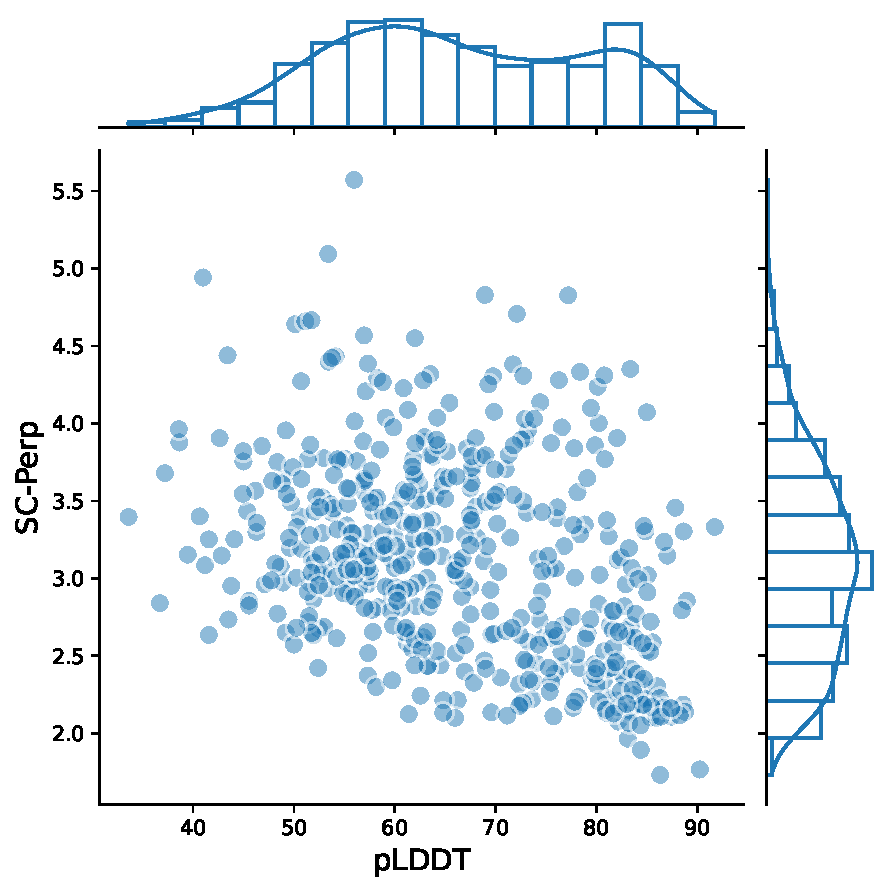
\includegraphics[scale=0.35]{images/plddt_scperp.pdf}
		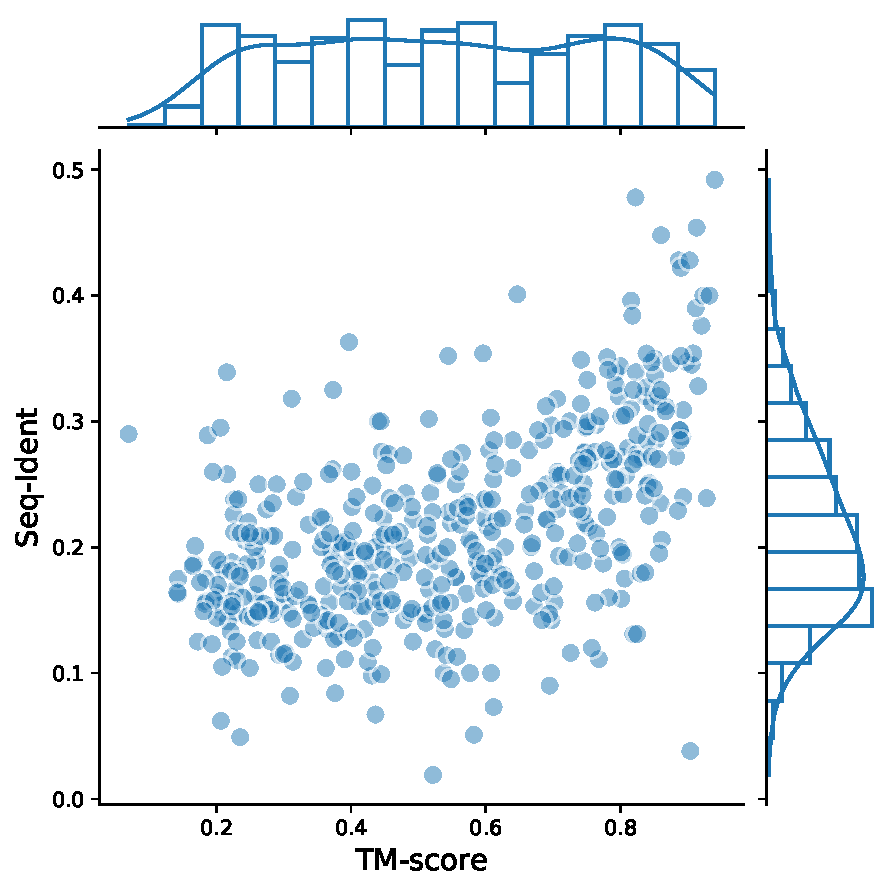
\includegraphics[scale=0.35]{images/tm_sid.pdf}
	\end{center}
	\credit{Image}{lv2024prollama}
	\begin{itemize}
		\item 1 spot = 1 sequence
	\end{itemize}
\end{frame}

\end{document}